\section{Hipercuádricas afines.}\label{Rel:Tema3}


\begin{ejercicio}\label{ej:5.3.1}
    Clasifica las hipercuádricas de un espacio afín euclídeo de dimensión 1.

    Tenemos que la forma cuadrática de toda hipercuádrica en cierto sistema de referencia euclídeo $\cc{R}$ es una de las siguientes:
    \begin{enumerate}
        \item $\frac{x^2}{a^2}=0$.

        Es un único punto doble, el origen.

        
        \item $\frac{x^2}{a^2}=1$.

        Son dos puntos, $x=\pm a$.
        
        \item $\frac{x^2}{a^2}=-1$.
        
        No es posible, por lo que es el vacío.
    \end{enumerate}
\end{ejercicio}


\begin{ejercicio}
    En el semiplano $P = \{(x, y, z) \in \bb{R}^3\mid y = 0, x \geq 0\}$ tomamos una circunferencia $C$ de centro $(c, 0, 0)$ y radio $r > 0$ con $c > r > 0$.
    Se llama toro de revolución generado por $C$ a la superficie $T$ obtenida al rotar $C$ alrededor del eje $z$.
    Dibujar $T$ y describir la superficie como el conjunto de soluciones de una ecuación con 3 incógnitas. ¿Es dicha ecuación la de una cuádrica?\\

    \begin{figure}[H]
        \centering
        \begin{tikzpicture}
          \begin{axis}[
              axis equal image,
              axis lines=middle,
              xmax=18,zmax=5,
              ticks=none,
              clip bounding box=upper bound,
              colormap/blackwhite
            ]
            % // TODO: Activar toro.
            %\addplot3[domain=0:360,y domain=0:320, samples=35,surf,z buffer=sort]
            %({(12 + 3 * cos(x)) * cos(y)} ,
            %{(12 + 3 * cos(x)) * sin(y)},
            %{3 * sin(x)});
            % use axis coordinate system to draw the radii
            \draw [thick,blue] (axis cs: 0,0,0) -- (axis cs: 12,0,0) node [midway, above] {$c$};
            \draw [thick,red] (axis cs: 12,-0.2,0) -- (axis cs: 12,3.7,0) node [midway, right, xshift=4pt] {$r$};
        
            % use axis coordinate system to draw fake x, y and z axes
            \draw [-latex] (axis cs: 0,0,0) -- node [pos=0.9, xshift=0.5em]{$z$}(axis cs: 0,0,10);
            \draw [-latex] (axis cs: 0,-15,0) -- (axis cs: 0,-20,0);
            \draw (axis cs: 0,0,0) -- (axis cs: 0,9,0);
            \draw (axis cs: 0,0,0) -- (axis cs: -9,0,0);
          \end{axis}
        \end{tikzpicture}
        \caption{Toro.}
        \label{fig:Toro}
    \end{figure}

    Veamos cuál es su ecuación. Para ello, fijado un punto $(x,y,z)\in \bb{R}^3$ que pertenezca al toro, realizamos un corte al toro por el plano 
        que pasa por dicho punto y es perpendicular al plano de ecuación $z=0$. Es decir, por el plano dado por $\pi:(x,y,z)+{\cc{L}\{(0,0,1)\}}^{\perp}$,
        y tenemos lo siguiente:
        \begin{figure}[H]
            \centering
            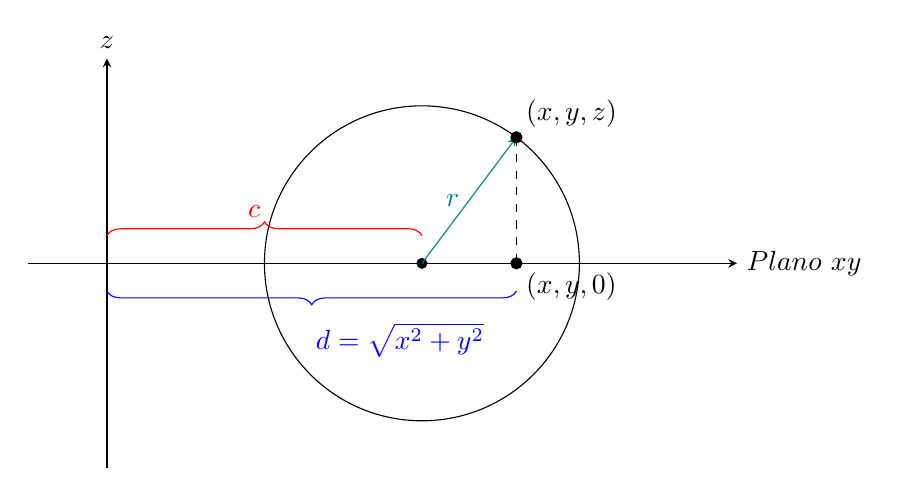
\begin{tikzpicture}[scale=2]
                % Eje horizontal
                \draw[-stealth] (-0.5,0) -- (4,0) node[right] {$Plano~xy$};
                % Eje vertical (A)
                \draw[-stealth] (0,-1.3) -- (0,1.3) node[above] {$z$};

                \def\r{1}
                \def\R{2}

                \coordinate (P) at (2.6,0.8);
                \coordinate (Q) at (2.6,0);
                \coordinate (O) at (\R,0);
                % Dibuja la circunferencia
                \draw (O) circle [radius=\r];
                % Marca el centro de la circunferencia
                \fill (O) circle [radius=1pt];% node[below] {$(2,0)$};
                
                % Etiqueta el radio
                \draw[-stealth, teal] (O) -- (P) node[midway, left] {$r$};
                % Punto en la circunferencia P(2.6,0.8)
                \filldraw (P) circle [radius=1pt] node[above right] {$(x,y,z)$};
                
                % Proyeccion del P
                \filldraw (Q) circle [radius=1pt] node[below right] {$(x,y,0)$};

                \draw[dashed] (P) -- (Q);

                % Cota con recta hacia abajo
                \draw[decorate,decoration={brace,amplitude=5pt,mirror},xshift=0pt,yshift=-5pt, blue]
                (0,0) -- (2.6,0) node[midway,below right,yshift=-8pt, xshift=-2pt] {$d=\sqrt{x^2+y^2}$};

                \draw[decorate,decoration={brace,amplitude=5pt},xshift=0pt,yshift=5pt, red]
                (0,0) -- (2,0) node[midway,above left,yshift=3pt, xshift=2pt] {$c$};
            \end{tikzpicture}
        \end{figure}
        donde sabemos que, por el teorma de Pitágoras, la distancia de $(x,y,0)$ al origen es $d=\sqrt{x^2+y^2}$. Por tanto, el punto $(x,y,z)\in \bb{R}^3$ estará en el toro de rotación de la circunferencia de radio $r$ a una distancia $c$ del eje de rotación $z$ si y solo si cumple el Teorema de Pitágoras del triángulo inscrito. Es decir:
        \begin{equation*}
            \left(\sqrt{x^2+y^2}-c\right)^2 + z^2= 1
        \end{equation*}

        Desarrollamos dicha ecuación para ver si se trata o no de una cuádrica:
        \begin{equation*}
            \begin{split}
                \left(\sqrt{x^2+y^2}-c\right)^2 + z^2&= 1\\
                x^2+y^2-2c\sqrt{x^2+y^2}+c^2+z^2&= 1\\
                x^2+y^2+z^2-2c\sqrt{x^2+y^2}+c^2-1&= 0
            \end{split}
        \end{equation*}

        Por tanto, como la ecuación asociada al Toro no es polinómica, no se trata de una cuádrica.
\end{ejercicio}


\begin{ejercicio}\label{ej:5.3.3}
    Sea $\cc{A}$ un espacio afín de dimensión $n$ y $S$ un subespacio afín suyo de dimensión $m > 0$. Demuestra que:
    \begin{enumerate}
        \item Existe un sistema de referencia $\cc{R}$ de $\cc{A}$ tal que las ecuaciones implícitas de $S$ en dicho sistema son $x_{m+1} = 0, \dots , x_n = 0$.
        
        Sea $S=p_0+\cc{L}\{v_1,\dots,v_m\} \subseteq \cc{A}$, con $p_0\in \cc{A}$ y $\{v_1,\dots,v_m\}$ una base de $\vec{S}$.
        Sea entonces el sistema de referencia buscado $\cc{R}=(p_0,\{v_1,\dots,v_m, v_{m+1},\dots, v_n\})$ un sistema de referencia de $\cc{A}$, donde $\{v_{m+1},\dots,v_n\}$ se han escogido extendiendo la base de $\vec{S}$ a una base de $\vec{\cc{A}}$.
        
        Las coordenadas en $\cc{R}$ de un punto $p\in \cc{A}$ son las coordenadas de $\vec{p_0p}$ en la base $\{v_1,\dots,v_m, v_{m+1},\dots, v_n\}$.
        Por tanto, si $p\in S$, entonces $\vec{p_0p}\in \vec{S}$, y por tanto es combinación lineal de los vectores de la base de $\vec{S}$. Es decir,
        \begin{equation*}
            \vec{p_0p}=\lambda_1v_1+\dots+\lambda_mv_m \qquad \lambda_1,\dots,\lambda_m\in \bb{R}
        \end{equation*}
        Por tanto, las coordenadas de $p$ en $\cc{R}$ son $(\lm_1, \dots, \lm_m, 0, \dots, 0)$, es decir, $x_{m+1}=\dots=x_n=0$.
        Debido a la unicidad de las coordenadas de un punto en un sistema de referencia, tenemos que las ecuaciones implícitas de $S$ en $\cc{R}$ son $x_{m+1}=\dots=x_n=0$.

        \item \label{item:5.3.3.b} Si $H$ es una hipercuádrica de $\cc{A}$, entonces $H \cap S$ es una hipercuádrica de $S$ o bien vacío o todo $S$.
        
        Sea $H$ una hipercuádrica de $\cc{A}$, y sea $\cc{R}$ un sistema de referencia de $\cc{A}$ tal que las ecuaciones implícitas de $S$ en $\cc{R}$ son $x_{m+1}=\dots=x_n=0$ (en el apartado anterior hemos visto que dicho sistema existe).
        Por tanto, si suponemos que la ecuación asociada a $H$ en $\cc{R}$ es $\sum\limits_{i,j=1}^n a_{ij}x_ix_j+\sum\limits_{i=1}^n b_ix_i+c=0$, tenemos que la ecuación asociada a $H\cap S$ en $\cc{R}$ es:
        \begin{equation*}
            \sum\limits_{i,j=1}^m a_{ij}x_ix_j+\sum\limits_{i=1}^m b_ix_i+c=0
        \end{equation*}

        Por tanto, por norma general, $H\cap S$ es una hipercuádrica de $S$. Veamos en qué casos no lo es distinguiendo:
        \begin{itemize}
            \item Por norma general, $H\cap S$ será una hipercuádrica de $\cc{S}$, ya que es una hipercuádrica de $\cc{A}$ y cumple las ecuaciones implícitas de $S$.
            \item Si $a_{ij}=b_i=0~\forall i,j\leq m$, $c\neq 0$, tenemos que la ecuación de la hipercuádrica es $c=0$, que es un absurdo, por lo que $H\cap S=\emptyset$.
            \item Si $a_{ij}=b_i=0~\forall i,j\leq m$, $c=0$, tenemos que la ecuación de $H\cap S$ es $0=0$, que es trivial, por lo que $H\cap S=S$.
        \end{itemize}
    \end{enumerate}
\end{ejercicio}



\begin{ejercicio}
    Sean $H$ una hipercuádrica y $R$ una recta de un espacio euclídeo $\cc{A}$.
    Prueba que $R \cap H$ puede ser vacío, un punto, dos puntos o toda la recta.
    Da un ejemplo conocido de cada uno de los casos cuando $\cc{A}$ tiene dimensión dimensión 2 y dimensión 3.\\

    En el Ejercicio \ref{ej:5.3.3}.\ref{item:5.3.3.b} hemos visto que $H\cap R$ es o bien el vacío, o bien $R$, o bien una hipercuádrica de $R$.
    Además, en el Ejercicio \ref{ej:5.3.1} hemos visto que las hipercuádricas de un espacio afín de dimensión 1 ($R$) son, o bien un punto, o bien dos puntos.
    Por tanto, tenemos que $H\cap R$ puede ser vacío, un punto, dos puntos o toda la recta, como queríamos demostrar.

    Veamos ahora un ejemplo de cada caso. En el caso de dimensión 2, fijemos $\cc{R}$ como sistema de referencia, y todas las ecuaciones implícitas vendrán dadas en dicho sistema $\cc{R}$.
    Consideremos el par de rectas secantes $H\equiv x^2-y^2=0$, que es una hipercuádrica. En el caso de $R_1\equiv y=0$, tenemos que $H\cap R_1=\{(0,0)_{\cc{R}}\}$, que es un punto.
    En el caso de $R_2\equiv y=1$, tenemos que $H\cap R_2=\{(1,1)_{\cc{R}}, (1,-1)_{\cc{R}}\}$, que son dos puntos.
    En el caso de $R_3\equiv x=y$, tenemos que $R_3\subset H$, por lo que $H\cap R_3=R_3$, que es toda la recta. Para el caso de intersección
    vacía, basta con tomar $H'\equiv y=x^2$ parábola y $R_4\equiv y=-1$, y tenemos que $H'\cap R_4=\emptyset$. 
    \begin{figure}[H]
        \begin{subfigure}{0.45\linewidth}
            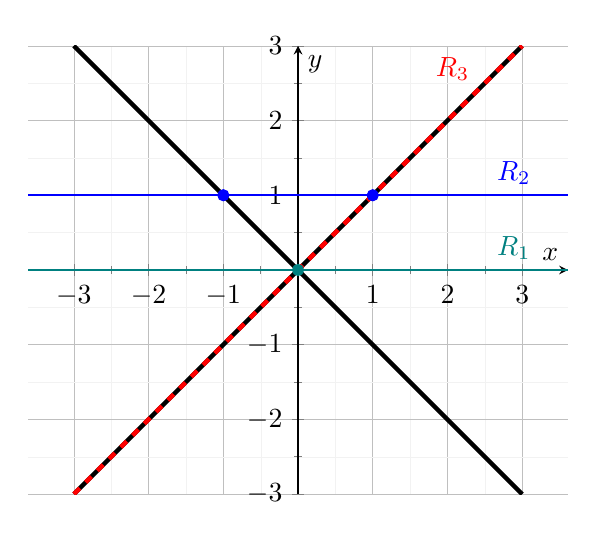
\begin{tikzpicture}
                \begin{axis}[
                    axis lines=center,
                    axis equal,
                    xlabel=$x$, ylabel=$y$,
                    xmin=-3, xmax=3,
                    ymin=-3, ymax=3,
                    xtick={-3,...,3},
                    ytick={-3,...,3},
                    grid=both,
                    grid style={line width=.1pt, draw=gray!10},
                    major grid style={line width=.2pt,draw=gray!50},
                    minor tick num=1,
                    clip=true
                ]   
                    % Hipercuádrica x^2-y^2=0
                    \addplot[ultra thick,domain=-3:3] {-x};
                    \addplot[ultra thick,domain=-3:3] {x};
    
    
                    % Recta x=0, junto con su punto de intersección con la hipercuádrica
                    \addplot[teal, thick, domain=-4:4] {0} node[above, xshift=-30pt] {$R_1$};
                    \addplot[only marks, teal,mark=*] coordinates {(0,0)};
    
                    % Recta x=1, junto con sus puntos de intersección con la hipercuádrica
                    \addplot[blue, thick,domain=-4:4] {1} node[above, xshift=-30pt] {$R_2$};
                    \addplot[only marks, blue,mark=*] coordinates {(-1,1) (1,1)};
    
                    % Recta x=y, junto con su punto de intersección con la hipercuádrica
                    \addplot[ultra thick, red, dashed, domain=-3:3] {x} node[below left, xshift=-15pt] {$R_3$};
                \end{axis}
            \end{tikzpicture}
        \end{subfigure}\hfill
        \begin{subfigure}{0.45\linewidth}
            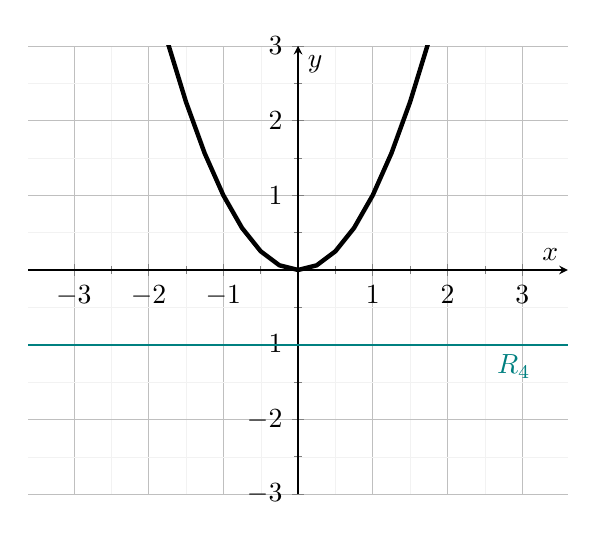
\begin{tikzpicture}
                \begin{axis}[
                    axis lines=center,
                    axis equal,
                    xlabel=$x$, ylabel=$y$,
                    xmin=-3, xmax=3,
                    ymin=-3, ymax=3,
                    xtick={-3,...,3},
                    ytick={-3,...,3},
                    grid=both,
                    grid style={line width=.1pt, draw=gray!10},
                    major grid style={line width=.2pt,draw=gray!50},
                    minor tick num=1,
                    clip=true
                ]   
                    % Hipercuádrica y=x^2
                    \addplot[ultra thick,domain=-3:3] {x^2};
    
    
                    % Recta y=-1
                    \addplot[thick, teal,domain=-4:4] {-1} node[below, xshift=-30pt] {$R_4$};
                \end{axis}
            \end{tikzpicture}
        \end{subfigure}
        \caption{Ejemplos de intersecciones de hipercuádricas con rectas en $\cc{A}^2$.}
    \end{figure}

    En el caso de dimensión 3, fijemos $\cc{R}$ como sistema de referencia, y todas las ecuaciones implícitas vendrán dadas en dicho sistema $\cc{R}$.
    Consideremos el par de planos secantes $H\equiv x^2-y^2=0$, que es una hipercuádrica. En el caso de $R_1\equiv x=z=0$, tenemos que $H\cap R_1=\{(0,0,0)_{\cc{R}}\}$, que es un punto.
    En el caso de $R_2\equiv x=z=1$, tenemos que $H\cap R_2=\{(1,1,1)_{\cc{R}}, (1,-1,1)_{\cc{R}}\}$, que son dos puntos.
    En el caso de $R_3\equiv x=y=0$, el eje $Z$, tenemos que $R_3\subset H$, por lo que $H\cap R_3=R_3$, que es toda la recta. Para el caso de intersección
    vacía, basta con tomar $H'\equiv y=x^2$ cilindro parabólico y $R_4\equiv y=x=-1$, y tenemos que $H'\cap R_4=\emptyset$.
\end{ejercicio}



\begin{ejercicio}
    Construir explícitamente un isomorfismo afín $f : \bb{R}^n \to \bb{R}^n$ tal que $f(C) = C'$ en cada uno de los siguientes casos:
    \begin{enumerate}
        \item $n=2$, $C=\left\{(x,y)\in \bb{R}^2\left|\dfrac{x^2}{a^2} + \dfrac{y^2}{b^2}=1\right.\right\}$, $C'=\left\{(x,y)\in \bb{R}^2\left|x^2 - y^2=1\right.\right\}$.
        
        En este caso, $C$ es una elipse y $C'$ una hipérbola. Como sabemos que estas no son equivalentes, tenemos que $\nexists f$ isomorfismo afín tal que $f(C)=C'$.
        % // TODO: No hay isomorfismo afín entre elipse e hipérbola.
        
        \item $n=3$, $C=\left\{(x,y,z)\in \bb{R}^3\left|x^2 + y^2+z^2=1\right.\right\}$, $C'=\left\{(x,y,z)\in \bb{R}^3\left|\dfrac{x^2}{a^2} + \dfrac{y^2}{b^2} + \dfrac{z^2}{c^2}=1\right.\right\}$.
        
        En ambos casos se trata de ellipsoides, por lo que es posible. Para ello, consideremos el isomorfismo afín $f:\bb{R}^3\to \bb{R}^3$ dado por:
        \begin{equation*}
            f(x,y,z) = \left(ax, bx, cz\right)
        \end{equation*}

        Veamos que $f(C)=C'$:
        \begin{description}
            \item[$\subset)$] Sea $(x,y,z)\in C$, y veamos que $f(x,y,z)\in C'$. Tenemos que:
            \begin{align*}
                f(x,y,z) &= \left(ax, bx, cz\right) \in C' \Longleftrightarrow \\ & \Longleftrightarrow
                 \frac{(ax)^2}{a^2} + \frac{(bx)^2}{b^2} + \frac{(cz)^2}{c^2} = x^2+y^2+z^2=1
            \end{align*}
            Y tenemos que es cierto, ya que $(x,y,z)\in C$.

            \item[$\supset)$] Sea $(x',y',z')\in C'$, y veamos que $\exists (x,y,z)\in C$ tal que su imagen es dicho punto, es decir, $f(x,y,z)=(x',y',z')$. Tenemos que:
            \begin{align*}
                (x',y',z')\in C' &\Longleftrightarrow
                \frac{(x')^2}{a^2} + \frac{(y')^2}{b^2} + \frac{(z')^2}{c^2} = 1 \Longleftrightarrow \\ & \Longleftrightarrow
                \left(\frac{x}{a}\right)^2 + \left(\frac{y}{b}\right)^2 + \left(\frac{z}{c}\right)^2 = 1 \Longleftrightarrow
                \left( \frac{x}{a}, \frac{y}{b}, \frac{z}{c} \right) \in C
            \end{align*}
        \end{description}

        \item $n=2$, $C=\left\{(x,y)\in \bb{R}^2\left|x^2-y=0\right.\right\}$, $C'=\left\{(x,y)\in \bb{R}^2\left|x-y^2=0\right.\right\}$.
        
        En este caso, ambos conjuntos son parábolas, por lo que es posible. Para ello, consideremos el isomorfismo afín $f:\bb{R}^2\to \bb{R}^2$ dado por:
        \begin{equation*}
            f(x,y) = (y,x)
        \end{equation*}

        Veamos que $f(C)=C'$:
        \begin{description}
            \item[$\subset)$] Sea $(x,y)\in C$, y veamos que $f(x,y)\in C'$. Tenemos que:
            \begin{align*}
                f(x,y) &= (y,x) \in C' \Longleftrightarrow
                 y - x^2 =  0 \Longleftrightarrow x^2-y=0
            \end{align*}
            Y tenemos que es cierto, ya que $(x,y)\in C$.

            \item[$\supset)$] Sea $(x',y')\in C'$, y veamos que $\exists (x,y)\in C$ tal que su imagen es dicho punto, es decir, $f(x,y)=(x',y')$. Tenemos que:
            \begin{align*}
                (x',y')\in C' &\Longleftrightarrow
                x' - (y')^2 = 0 \Longleftrightarrow
                (y')^2 -x = 0 \Longleftrightarrow
                (y',x') \in C
            \end{align*}
        \end{description}

        \item $n=3$, $C=\left\{(x,y,z)\in \bb{R}^3\left|ax^2+by^2=1\right.\right\}$, $C'=\left\{(x,y,z)\in \bb{R}^3\left|x^2+y^2=1\right.\right\}$.
        
        Suponemos que $a,b\in \bb{R}^+$, ya que si no, $C$ no es un cilindro elíptico y, como $C'$ sí lo es, no existiría tal isomorfismo afín.
        Por tanto, en dicha suposición, consideremos el isomorfismo afín $f:\bb{R}^3\to \bb{R}^3$ dado por:
        \begin{equation*}
            f(x,y,z) = \left(\sqrt{a}x , \sqrt{b}y, z\right)
        \end{equation*}

        Veamos que $f(C)=C'$:
        \begin{description}
            \item[$\subset)$] Sea $(x,y,z)\in C$, y veamos que $f(x,y,z)\in C'$. Tenemos que:
            \begin{align*}
                f(x,y,z) &= \left(\sqrt{a}x , \sqrt{b}y, z\right) \in C' \Longleftrightarrow \\ & \Longleftrightarrow
                 (\sqrt{a}x)^2 + (\sqrt{b}y)^2 = a x^2 + b y^2 = 1
            \end{align*}
            Y tenemos que es cierto, ya que $(x,y,z)\in C$.

            \item[$\supset)$] Sea $(x',y',z')\in C'$, y veamos que $\exists (x,y,z)\in C$ tal que su imagen es dicho punto, es decir, $f(x,y,z)=(x',y',z')$. Tenemos que:
            \begin{align*}
                (x',y',z')\in C' &\Longleftrightarrow
                (x')^2 + (y')^2 = 1 \Longleftrightarrow \\ & \Longleftrightarrow
                \left(x'\cdot \frac{\sqrt{a}}{\sqrt{a}}\right)^2 + \left(y'\cdot \frac{\sqrt{b}}{\sqrt{b}}\right)^2 = 1 \Longleftrightarrow \\ & \Longleftrightarrow
                \left(\frac{x'}{\sqrt{a}}, \frac{y'}{\sqrt{b}}, z'\right) \in C
            \end{align*}
        \end{description}

    \end{enumerate}
\end{ejercicio}



\begin{ejercicio} Cuestiones sobre elipses:
\begin{enumerate}
    \item Dados dos puntos distintos $p_1, p_2$ de un plano afín euclídeo $\bb{E}$ y $r > d(p_1, p_2)$, demuestra que $H=\{p \in \bb{E} \mid d(p, p_1) + d(p, p_2) = r\}$ es una elipse.
    Los puntos $p_1, p_2$ reciben el nombre de focos de la elipse.
    Se llama centro de la elipse al punto medio de sus focos y vértices a los puntos de intersección de la elipse
    con la recta que pasa por sus focos.

    \begin{figure}[H]
        \centering
        \begin{tikzpicture}
            % Origen
            \coordinate (O) at (0,0);

            % Focos
            \coordinate (F1) at (-2,0);
            \coordinate (F2) at (2,0);

            % Punto de la elipse
            \coordinate (P) at (1.5,1.2);

            % Eje menor
            \coordinate (Eje_Menor_init) at (0,2);
            \coordinate (Eje_Menor_end) at (0,-2);

            % Eje mayor
            \coordinate (Eje_Mayor_init) at (-3,0);
            \coordinate (Eje_Mayor_end) at (3,0);

            % Vectores que unen P con los focos
            \coordinate (P_F1) at ($(P)-(F1)$);
            \coordinate (P_F2) at ($(P)-(F2)$);

            % Vector v1 y v2
            \coordinate (v1) at (1, 0);
            \coordinate (v2) at (0, 1);

            % Dibujamos los ejes
            \draw[dashed] (Eje_Menor_init) -- (Eje_Menor_end);
            \draw[dashed] (Eje_Mayor_init) -- (Eje_Mayor_end);

            % Dibujamos los focos
            \fill (F1) circle [radius=1pt] node[below right] {$p_1$};
            \fill (F2) circle [radius=1pt] node[below left] {$p_2$};

            % Dibujamos el punto de la elipse
            \fill (P) circle [radius=1pt] node[above right] {$p$};

            % Dibujamos los vectores que unen P con los focos
            \draw[thick, red, -stealth] (F1) -- (P) node[midway, above left] {$\vec{p_1p}$};
            \draw[thick, red, -stealth] (F2) -- (P) node[midway, above right, xshift=4pt] {$\vec{p_2p}$};

            % Dibujamos el vector v1 y v2
            \draw[blue, -stealth] (O) -- (v1) node[midway, below] {$v_1$};
            \draw[blue, -stealth] (O) -- (v2) node[midway, right] {$v_2$};

            % Dibujamos la elipse
            \draw[thick, teal] (O) ellipse (2.5cm and 1.5cm);
        \end{tikzpicture}
        \caption{Elipse de focos $p_1$ y $p_2$.}  
        \label{fig:ej5.3.6.Elipse}      
    \end{figure}
    Sea el vector unitario $v_1=\dfrac{\vec{p_1p_2}}{\left\|\vec{p_1p_2}\right\|}\in \vec{\bb{E}}$, y sea $v_2\in \vec{\bb{E}}$ tal que $\cc{B}=\{v_1,v_2\}$ es una base ortonormal orientada positivamente (estos vectores están representados también el la Figura \ref{fig:ej5.3.6.Elipse}).
    Consideramos el sistema de referencia ortonormal $\cc{R}=\{m_{p_1p_2},\cc{B}\}$. Calculamos las coordenadas de $p_1$ y $p_2$ en $\cc{R}$:
    \begin{align*}
        p_1 &= m_{p_1p_2} - \frac{\vec{p_1p_2}}{2} = m_{p_1p_2} - \frac{\left\|\vec{p_1p_2}\right\|}{2}\cdot \frac{\vec{p_1p_2}}{\left\|\vec{p_1p_2}\right\|} = \left(-\frac{\left\|\vec{p_1p_2}\right\|}{2}, 0\right)_{\cc{R}} \\
        p_2 &= m_{p_1p_2} + \frac{\vec{p_1p_2}}{2} = m_{p_1p_2} + \frac{\left\|\vec{p_1p_2}\right\|}{2}\cdot \frac{\vec{p_1p_2}}{\left\|\vec{p_1p_2}\right\|} = \left(\frac{\left\|\vec{p_1p_2}\right\|}{2}, 0\right)_{\cc{R}}
    \end{align*}

    Sea entonces $p\in H$, con $p=(x,y)_{\cc{R}}$. Tenemos que:
    \begin{align*}
        p\in H &\Longleftrightarrow
        d(p,p_1) + d(p,p_2) = r \Longleftrightarrow \\ & \Longleftrightarrow
        \sqrt{\left(x+\frac{\left\|\vec{p_1p_2}\right\|}{2}\right)^2 + y^2} + \sqrt{\left(x-\frac{\left\|\vec{p_1p_2}\right\|}{2}\right)^2 + y^2} = r \Longleftrightarrow \\ & \Longleftrightarrow
        \sqrt{\left(x+\frac{\left\|\vec{p_1p_2}\right\|}{2}\right)^2 + y^2} = r - \sqrt{\left(x-\frac{\left\|\vec{p_1p_2}\right\|}{2}\right)^2 + y^2} \Longleftrightarrow \\ & \Longleftrightarrow
        \left(x+\frac{\left\|\vec{p_1p_2}\right\|}{2}\right)^2 + y^2 = \left(r - \sqrt{\left(x-\frac{\left\|\vec{p_1p_2}\right\|}{2}\right)^2 + y^2}\right)^2 \Longleftrightarrow \\ & \Longleftrightarrow
        \left(x+\frac{\left\|\vec{p_1p_2}\right\|}{2}\right)^2 + \cancel{y^2} =\\&\hspace{2cm}=r^2 - 2r\sqrt{\left(x-\frac{\left\|\vec{p_1p_2}\right\|}{2}\right)^2 + y^2} + \left(x-\frac{\left\|\vec{p_1p_2}\right\|}{2}\right)^2 + \cancel{y^2} \Longleftrightarrow \\ & \Longleftrightarrow
        \left(x+\frac{\left\|\vec{p_1p_2}\right\|}{2}\right)^2 - \left(x-\frac{\left\|\vec{p_1p_2}\right\|}{2}\right)^2 =r^2 - 2r\sqrt{\left(x-\frac{\left\|\vec{p_1p_2}\right\|}{2}\right)^2 + y^2} \stackrel{(\ast)}{\Longleftrightarrow} \\ & \stackrel{(\ast)}{\Longleftrightarrow}
        2x\left\|\vec{p_1p_2}\right\| = r^2 - 2r\sqrt{\left(x-\frac{\left\|\vec{p_1p_2}\right\|}{2}\right)^2 + y^2} \Longleftrightarrow \\ & \Longleftrightarrow
        r^2 - 2x\left\|\vec{p_1p_2}\right\| = 2r\sqrt{\left(x-\frac{\left\|\vec{p_1p_2}\right\|}{2}\right)^2 + y^2} \Longleftrightarrow \\ & \Longleftrightarrow
        r^4 + 4x^2\left\|\vec{p_1p_2}\right\|^2 - 4r^2x\left\|\vec{p_1p_2}\right\| = 4r^2\left(x-\frac{\left\|\vec{p_1p_2}\right\|}{2}\right)^2 + 4r^2y^2 \Longleftrightarrow \\ & \Longleftrightarrow
        r^4 + 4x^2\left\|\vec{p_1p_2}\right\|^2 - 4r^2x\left\|\vec{p_1p_2}\right\| =\\&\hspace{2cm}=4r^2x^2 - 4r^2x\left\|\vec{p_1p_2}\right\| +r^2\left\|\vec{p_1p_2}\right\|^2 + 4r^2y^2 \Longleftrightarrow \\ & \Longleftrightarrow
        r^4 + 4x^2\left(\left\|\vec{p_1p_2}\right\|^2-r^2\right) -\cancel{4r^2x\left\|\vec{p_1p_2}\right\|} =\\&\hspace{2cm}= - \cancel{4r^2x\left\|\vec{p_1p_2}\right\|} +r^2\left\|\vec{p_1p_2}\right\|^2 + 4r^2y^2 \Longleftrightarrow \\ & \Longleftrightarrow
        4x^2\left(r^2 - \left\|\vec{p_1p_2}\right\|^2\right) + 4r^2y^2 = r^2\left(r^2 - \left\|\vec{p_1p_2}\right\|^2\right)
    \end{align*}
    donde en $(\ast)$ he aplicado que $a^2-b^2=(a+b)(a-b)$. Para que sea una alipse, es necesario que:
    \begin{equation*}
        r^2 - \left\|\vec{p_1p_2}\right\|^2 > 0 \Longleftrightarrow
        r^2 > \left\|\vec{p_1p_2}\right\|^2 \Longleftrightarrow
        r > \left\|\vec{p_1p_2}\right\|
    \end{equation*}
    que es cierto por hipótesis. Tenemos por tanto que, efectivamente, $H$ es una elipse.
    
    Notando $r=2a$, $c=\frac{1}{2}\left\|\vec{p_1p_2}\right\|$ y $b=\sqrt{a^2-c^2}$, tenemos que:
    \begin{align*}
        p\in H &\Longleftrightarrow 4x^2\left(4a^2 - 4c^2\right) + 4\cdot 4a^2y^2 = 4a^2(4a^2 - 4c^2) \Longleftrightarrow \\ & \Longleftrightarrow
        4x^2b^2 + 4a^2y^2 = 4a^2b^2 \Longleftrightarrow
        \frac{x^2}{a^2} + \frac{y^2}{b^2} = 1
    \end{align*}

    El valor $c$ recibe el nombre de distancia focal de la elipse, y el valor de $a$ se denomina semieje mayor de la elipse.
    El valor de $b$ se denomina semieje menor de la elipse.

    \item Prueba que toda elipse se puede escribir como en el apartado anterior, para ciertos puntos $p_1, p_2 \in \bb{E}$.
    
    Sabemos que toda elipse, en cierto sistema de referencia ortonormal $\cc{R}$ dado por $\cc{R}=~\{p_0, \{v_1, v_2\}\}$, tiene como ecuación asociada en $\cc{R}$:
    \begin{equation*}
        \frac{x^2}{a^2} + \frac{y^2}{b^2} = 1 \qquad \text{con } a,b\in \bb{R}^+,~a\geq b
    \end{equation*}

    Sea $c=\sqrt{a^2-b^2}$, y sea $p_1 = p_0 - c\cdot v_1=(-c,0)_{\cc{R}}$ y $p_2 = p_0  +c\cdot v_1=(c,0)_{\cc{R}}$. Tenemos que:
    \begin{equation*}
        \left\|\vec{p_1p_2}\right\| = \left\|p_2 - p_1\right\| = \left\|2c\cdot v_1\right\|= 2c \Longrightarrow c = \frac{1}{2}\left\|\vec{p_1p_2}\right\|
    \end{equation*}

    Por tanto, definiendo $r=2a$, y como en el apartado anterior
    eran dobles implicaciones, tenemos que:
    \begin{equation*}
        p\in H \Longleftrightarrow \frac{x^2}{a^2} + \frac{y^2}{b^2} = 1
        \Longleftrightarrow d(p,p_1) + d(p,p_2) = r
    \end{equation*}

    \item Demuestra que toda elipse $H$ es simétrica con respecto a la recta $R_{p_1p_2}$ que pasa por sus focos (denominada eje mayor) y con respecto a la mediatriz de sus focos (denominado eje menor).
    
    Sea el vector unitario $v_1=\dfrac{\vec{p_1p_2}}{\left\|\vec{p_1p_2}\right\|}\in \vec{\bb{E}}$, y sea $v_2\in \vec{\bb{E}}$ tal que $\cc{B}=\{v_1,v_2\}$ es una base ortonormal orientada positivamente (estos vectores están representados también el la Figura \ref{fig:ej5.3.6.Elipse}).
    Consideramos el sistema de referencia ortonormal $\cc{R}=\{m_{p_1p_2},\cc{B}\}$. Tenemos que las coordenadas de $p_1$ y $p_2$ en $\cc{R}$ son:
    \begin{equation*}
        p_1 = \left(-\frac{\left\|\vec{p_1p_2}\right\|}{2}, 0\right)_{\cc{R}} \qquad
        p_2 = \left(\frac{\left\|\vec{p_1p_2}\right\|}{2}, 0\right)_{\cc{R}}
    \end{equation*}

    Sea entonces $p\in \bb{E}$, con $p=(x,y)_{\cc{R}}$. Tenemos que:
    \begin{equation*}
        \sigma_{R_{p_1p_2}}(p)= (x,-y)_{\cc{R}}
    \end{equation*}
    donde he usado que $R_{p_1p_2}=p_1+\cc{L}\{v_1\}$ por la definición de $v_1$.

    Por tanto, tenemos que:
    \begin{align*}
        d(p, p_1)& + d(p, p_2) = d((x,y), p_1) + d((x,y), p_2)\\&
        = \sqrt{\left(x+\frac{\left\|\vec{p_1p_2}\right\|}{2}\right)^2 + y^2} + \sqrt{\left(x-\frac{\left\|\vec{p_1p_2}\right\|}{2}\right)^2 + y^2} = \\&
        = \sqrt{\left(x+\frac{\left\|\vec{p_1p_2}\right\|}{2}\right)^2 + (-y)^2} + \sqrt{\left(x-\frac{\left\|\vec{p_1p_2}\right\|}{2}\right)^2 + (-y)^2} = \\ &
        = d((x,-y), p_1) + d((x,-y), p_2) = d(\sigma_{R_{p_1p_2}}(p), p_1) + d(\sigma_{R_{p_1p_2}}(p), p_2)
    \end{align*}

    Por tanto, $p\in H \Longleftrightarrow \sigma_{R_{p_1p_2}}(p)\in H$, es decir, $H$ es simétrica con respecto a $R_{p_1p_2}$.
    De forma análoga, notando por $M_{p_1p_2}={R_{p_1p_2}}^\perp_{m_{p_1p_2}}$ a la mediatriz del segmento $[p_1, p_2]$, tenemos que:
    \begin{equation*}
        \sigma_{M_{p_1p_2}}(p)= (-x,y)_{\cc{R}}
    \end{equation*}
    donde he usado que $M_{p_1p_2}=m_{p_1p_2}+\cc{L}\{v_2\}$ por la definición de $v_2$. Por tanto, tenemos que:
    \begin{align*}
        d(p, p_1)& + d(p, p_2) = d((x,y), p_1) + d((x,y), p_2)\\&
        = \sqrt{\left(x+\frac{\left\|\vec{p_1p_2}\right\|}{2}\right)^2 + y^2} + \sqrt{\left(x-\frac{\left\|\vec{p_1p_2}\right\|}{2}\right)^2 + y^2} =\\&
        = \sqrt{\left[-\left(x+\frac{\left\|\vec{p_1p_2}\right\|}{2}\right)\right]^2 + y^2} + \sqrt{\left[-\left(x-\frac{\left\|\vec{p_1p_2}\right\|}{2}\right)\right]^2 + y^2} = \\ &
        = \sqrt{\left(-x+\frac{\left\|\vec{p_1p_2}\right\|}{2}\right)^2 + y^2} + \sqrt{\left(-x-\frac{\left\|\vec{p_1p_2}\right\|}{2}\right)^2 + y^2} = \\ &
        = d((-x,y), p_1) + d((-x,y), p_2) = d(\sigma_{M_{p_1p_2}}(p), p_1) + d(\sigma_{M_{p_1p_2}}(p), p_2)
    \end{align*}

    Por tanto, $p\in H \Longleftrightarrow \sigma_{M_{p_1p_2}}(p)\in H$, es decir, $H$ es simétrica con respecto a $M_{p_1p_2}$.

    \item Prueba que, para cada punto $p$ de una elipse $H$, la recta tangente a $H$ en $p$ forma ángulos iguales con las rectas que pasan por $p$ y cada uno de sus focos.
    % // TODO: Tangente a elipse
\end{enumerate}
\end{ejercicio}



\begin{ejercicio} Cuestiones sobre hipérbolas:
\begin{enumerate}
    \item Dados dos puntos distintos $p_1, p_2$ de un plano afín euclídeo $\bb{E}$ y $r < d(p_1, p_2)$, demuestra que $H=\{p \in \bb{E} \mid |d(p, p_1) - d(p, p_2)| = r\}$ es una hipérbola.
    Los puntos $p_1, p_2$ reciben el nombre de focos de la hipérbola.
    Se llama centro de la hipérbola al punto medio de sus focos y vértices a los puntos de intersección de la hipérbola con la recta que pasa por sus focos.
    \begin{figure}[H]
        \centering
        \begin{tikzpicture}
            % Origen
            \coordinate (O) at (0,0);

            % Calcula raiz de 2
            \pgfmathsetmacro{\raiz}{sqrt(2)}

            % Focos
            \coordinate (F2) at (\raiz,0);
            \coordinate (F1) at (-\raiz,0);

            % Punto de la elipse
            \coordinate (P) at (1.95,1.7);

            % Eje menor
            \coordinate (Eje_Menor_init) at (0,2);
            \coordinate (Eje_Menor_end) at (0,-2);

            % Eje mayor
            \coordinate (Eje_Mayor_init) at (-3,0);
            \coordinate (Eje_Mayor_end) at (3,0);

            % Vectores que unen P con los focos
            \coordinate (P_F1) at ($(P)-(F1)$);
            \coordinate (P_F2) at ($(P)-(F2)$);

            % Vector v1 y v2
            \coordinate (v1) at (0.75, 0);
            \coordinate (v2) at (0, 0.75);

            % Dibujamos los ejes
            \draw[dashed] (Eje_Menor_init) -- (Eje_Menor_end);
            \draw[dashed] (Eje_Mayor_init) -- (Eje_Mayor_end);

            % Dibujamos los focos
            \fill (F1) circle [radius=1pt] node[below right] {$p_1$};
            \fill (F2) circle [radius=1pt] node[below left] {$p_2$};

            % Dibujamos el punto de la elipse
            \fill (P) circle [radius=1pt] node[above] {$p$};

            % Dibujamos los vectores que unen P con los focos
            \draw[thick, red, -stealth] (F1) -- (P) node[midway, right] {$\vec{p_1p}$};
            \draw[thick, red, -stealth] (F2) -- (P) node[midway, above] {$\vec{p_2p}$};

            % Dibujamos el vector v1 y v2
            \draw[blue, -stealth] (O) -- (v1) node[midway, below] {$v_1$};
            \draw[blue, -stealth] (O) -- (v2) node[midway, right] {$v_2$};

            % Dibujamos la hipérbola
            \def\a{1}
            \def\b{1}

            \draw[teal] plot[domain={-sqrt(\a^2 + 1)}:{sqrt(\a^2 + 1)}, samples=50] ({\a*cosh(\x)}, {\b*sinh(\x)});
            \draw[teal] plot[domain={-sqrt(\a^2 + 1)}:{sqrt(\a^2 + 1)}, samples=50] ({-\a*cosh(\x)}, {\b*sinh(\x)});

        \end{tikzpicture}
        \caption{Hipérbola de focos $p_1$ y $p_2$.}  
        \label{fig:ej5.3.7.Hiperbola}      
    \end{figure}
    Sea el vector unitario $v_1=\dfrac{\vec{p_1p_2}}{\left\|\vec{p_1p_2}\right\|}\in \vec{\bb{E}}$, y sea $v_2\in \vec{\bb{E}}$ tal que $\cc{B}=\{v_1,v_2\}$ es una base ortonormal orientada positivamente (estos vectores están representados también el la Figura \ref{fig:ej5.3.7.Hiperbola}).
    Consideramos el sistema de referencia ortonormal $\cc{R}=\{m_{p_1p_2},\cc{B}\}$. Calculamos las coordenadas de $p_1$ y $p_2$ en $\cc{R}$:
    \begin{align*}
        p_1 &= m_{p_1p_2} - \frac{\vec{p_1p_2}}{2} = m_{p_1p_2} - \frac{\left\|\vec{p_1p_2}\right\|}{2}\cdot \frac{\vec{p_1p_2}}{\left\|\vec{p_1p_2}\right\|} = \left(-\frac{\left\|\vec{p_1p_2}\right\|}{2}, 0\right)_{\cc{R}} \\
        p_2 &= m_{p_1p_2} + \frac{\vec{p_1p_2}}{2} = m_{p_1p_2} + \frac{\left\|\vec{p_1p_2}\right\|}{2}\cdot \frac{\vec{p_1p_2}}{\left\|\vec{p_1p_2}\right\|} = \left(\frac{\left\|\vec{p_1p_2}\right\|}{2}, 0\right)_{\cc{R}}
    \end{align*}

    Sea entonces $p\in H$, con $p=(x,y)_{\cc{R}}$. Tenemos que:
    \begin{align*}
        p\in H &\Longleftrightarrow
        d(p,p_1) - d(p,p_2) = \pm r \Longleftrightarrow \\ & \Longleftrightarrow
        \sqrt{\left(x+\frac{\left\|\vec{p_1p_2}\right\|}{2}\right)^2 + y^2} - \sqrt{\left(x-\frac{\left\|\vec{p_1p_2}\right\|}{2}\right)^2 + y^2} = \pm r \Longleftrightarrow \\ & \Longleftrightarrow
        \sqrt{\left(x+\frac{\left\|\vec{p_1p_2}\right\|}{2}\right)^2 + y^2} = \pm r + \sqrt{\left(x-\frac{\left\|\vec{p_1p_2}\right\|}{2}\right)^2 + y^2} \Longleftrightarrow \\ & \Longleftrightarrow
        \left(x+\frac{\left\|\vec{p_1p_2}\right\|}{2}\right)^2 + y^2 = \left(\pm r + \sqrt{\left(x-\frac{\left\|\vec{p_1p_2}\right\|}{2}\right)^2 + y^2}\right)^2 \Longleftrightarrow \\ & \Longleftrightarrow
        \left(x+\frac{\left\|\vec{p_1p_2}\right\|}{2}\right)^2 + \cancel{y^2} =\\&\hspace{2cm}=r^2 \pm  2r\sqrt{\left(x-\frac{\left\|\vec{p_1p_2}\right\|}{2}\right)^2 + y^2} + \left(x-\frac{\left\|\vec{p_1p_2}\right\|}{2}\right)^2 + \cancel{y^2} \Longleftrightarrow \\ & \Longleftrightarrow
        \left(x+\frac{\left\|\vec{p_1p_2}\right\|}{2}\right)^2 - \left(x-\frac{\left\|\vec{p_1p_2}\right\|}{2}\right)^2 =r^2 \pm 2r\sqrt{\left(x-\frac{\left\|\vec{p_1p_2}\right\|}{2}\right)^2 + y^2} \stackrel{(\ast)}{\Longleftrightarrow} \\ & \stackrel{(\ast)}{\Longleftrightarrow}
        2x\left\|\vec{p_1p_2}\right\| = r^2 \pm 2r\sqrt{\left(x-\frac{\left\|\vec{p_1p_2}\right\|}{2}\right)^2 + y^2} \Longleftrightarrow \\ & \Longleftrightarrow
        r^2 - 2x\left\|\vec{p_1p_2}\right\| = \mp 2r\sqrt{\left(x-\frac{\left\|\vec{p_1p_2}\right\|}{2}\right)^2 + y^2} \Longleftrightarrow \\ & \Longleftrightarrow
        r^4 + 4x^2\left\|\vec{p_1p_2}\right\|^2 - 4r^2x\left\|\vec{p_1p_2}\right\| = 4r^2\left(x-\frac{\left\|\vec{p_1p_2}\right\|}{2}\right)^2 + 4r^2y^2 \Longleftrightarrow \\ & \Longleftrightarrow
        r^4 + 4x^2\left\|\vec{p_1p_2}\right\|^2 - 4r^2x\left\|\vec{p_1p_2}\right\| =\\&\hspace{2cm}=4r^2x^2 - 4r^2x\left\|\vec{p_1p_2}\right\| +r^2\left\|\vec{p_1p_2}\right\|^2 + 4r^2y^2 \Longleftrightarrow \\ & \Longleftrightarrow
        r^4 + 4x^2\left(\left\|\vec{p_1p_2}\right\|^2-r^2\right) -\cancel{4r^2x\left\|\vec{p_1p_2}\right\|} =\\&\hspace{2cm}= - \cancel{4r^2x\left\|\vec{p_1p_2}\right\|} +r^2\left\|\vec{p_1p_2}\right\|^2 + 4r^2y^2 \Longleftrightarrow \\ & \Longleftrightarrow
        4x^2\left(r^2 - \left\|\vec{p_1p_2}\right\|^2\right) + 4r^2y^2 = r^2\left(r^2 - \left\|\vec{p_1p_2}\right\|^2\right)
    \end{align*}
    donde en $(\ast)$ he aplicado que $a^2-b^2=(a+b)(a-b)$. Para que sea una hipérbola, es necesario que:
    \begin{equation*}
        r^2 - \left\|\vec{p_1p_2}\right\|^2 < 0 \Longleftrightarrow
        r^2 < \left\|\vec{p_1p_2}\right\|^2 \Longleftrightarrow
        r < \left\|\vec{p_1p_2}\right\|
    \end{equation*}
    que es cierto por hipótesis. Tenemos por tanto que, efectivamente, $H$ es una hipérbola.

    Notando $r=2a$, $c=\frac{1}{2}\left\|\vec{p_1p_2}\right\|$ y $b=\sqrt{c^2-a^2}$, tenemos que:
    \begin{align*}
        p\in H &\Longleftrightarrow 4x^2\left(4a^2 - 4c^2\right) + 4\cdot 4a^2y^2 = 4a^2(4c^2 - 4a^2) \Longleftrightarrow \\ & \Longleftrightarrow
        -4x^2b^2 + 4a^2y^2 = -4a^2b^2 \Longleftrightarrow
        \frac{x^2}{a^2} - \frac{y^2}{b^2} = 1
    \end{align*}

    El valor $c$ recibe el nombre de distancia focal de la hipérbola, y el valor de $a$ se denomina semieje real (o mayor) de la hipérbola.
    El valor de $b$ se denomina semieje imaginario (o menor) de la hipérbola.

    \item Prueba que toda hipérbola se puede escribir como en el apartado anterior, para ciertos puntos $p_1, p_2 \in \bb{E}$.
    
    Sabemos que toda hipérbola, en cierto sistema de referencia ortonormal $\cc{R}$ dado por $\cc{R}=~\{p_0, \{v_1, v_2\}\}$, tiene como ecuación asociada en $\cc{R}$:
    \begin{equation*}
        \frac{x^2}{a^2} - \frac{y^2}{b^2} = 1 \qquad \text{con } a,b\in \bb{R}^+
    \end{equation*}

    Sea $c=\sqrt{a^2+b^2}$, y sea $p_1 = p_0 - c\cdot v_1=(-c,0)_{\cc{R}}$ y $p_2 = p_0  +c\cdot v_1=(c,0)_{\cc{R}}$. Tenemos que:
    \begin{equation*}
        \left\|\vec{p_1p_2}\right\| = \left\|p_2 - p_1\right\| = \left\|2c\cdot v_1\right\|= 2c \Longrightarrow c = \frac{1}{2}\left\|\vec{p_1p_2}\right\|
    \end{equation*}

    Por tanto, definiendo $r=2a$, y como en el apartado anterior eran dobles implicaciones, tenemos que:
    \begin{equation*}
        p\in H \Longleftrightarrow \frac{x^2}{a^2} - \frac{y^2}{b^2} = 1
        \Longleftrightarrow d(p,p_1) - d(p,p_2) = \pm r
    \end{equation*}


    \item  Demuestra que toda hipérbola $H$ es simétrica con respecto a la recta $R_{p_1p_2}$ que pasa por sus focos y con respecto a la mediatriz de sus focos.
    
    Sea el vector unitario $v_1=\dfrac{\vec{p_1p_2}}{\left\|\vec{p_1p_2}\right\|}\in \vec{\bb{E}}$, y sea $v_2\in \vec{\bb{E}}$ tal que $\cc{B}=\{v_1,v_2\}$ es una base ortonormal orientada positivamente (estos vectores están representados también el la Figura \ref{fig:ej5.3.7.Hiperbola}).
    Consideramos el sistema de referencia ortonormal $\cc{R}=\{m_{p_1p_2},\cc{B}\}$. Tenemos que las coordenadas de $p_1$ y $p_2$ en $\cc{R}$ son:
    \begin{equation*}
        p_1 = \left(-\frac{\left\|\vec{p_1p_2}\right\|}{2}, 0\right)_{\cc{R}} \qquad
        p_2 = \left(\frac{\left\|\vec{p_1p_2}\right\|}{2}, 0\right)_{\cc{R}}
    \end{equation*}

    Sea entonces $p\in \bb{E}$, con $p=(x,y)_{\cc{R}}$. Tenemos que:
    \begin{equation*}
        \sigma_{R_{p_1p_2}}(p)= (x,-y)_{\cc{R}}
    \end{equation*}
    donde he usado que $R_{p_1p_2}=p_1+\cc{L}\{v_1\}$ por la definición de $v_1$.

    Por tanto, tenemos que:
    \begin{align*}
        d(p, p_1)& + d(p, p_2) = d((x,y), p_1) + d((x,y), p_2)\\&
        = \sqrt{\left(x+\frac{\left\|\vec{p_1p_2}\right\|}{2}\right)^2 + y^2} + \sqrt{\left(x-\frac{\left\|\vec{p_1p_2}\right\|}{2}\right)^2 + y^2} = \\&
        = \sqrt{\left(x+\frac{\left\|\vec{p_1p_2}\right\|}{2}\right)^2 + (-y)^2} + \sqrt{\left(x-\frac{\left\|\vec{p_1p_2}\right\|}{2}\right)^2 + (-y)^2} = \\ &
        = d((x,-y), p_1) + d((x,-y), p_2) = d(\sigma_{R_{p_1p_2}}(p), p_1) + d(\sigma_{R_{p_1p_2}}(p), p_2)
    \end{align*}

    Por tanto, $p\in H \Longleftrightarrow \sigma_{R_{p_1p_2}}(p)\in H$, es decir, $H$ es simétrica con respecto a $R_{p_1p_2}$.
    De forma análoga, notando por $M_{p_1p_2}={R_{p_1p_2}}^\perp_{m_{p_1p_2}}$ a la mediatriz del segmento $[p_1, p_2]$, tenemos que:
    \begin{equation*}
        \sigma_{M_{p_1p_2}}(p)= (-x,y)_{\cc{R}}
    \end{equation*}
    donde he usado que $M_{p_1p_2}=m_{p_1p_2}+\cc{L}\{v_2\}$ por la definición de $v_2$. Por tanto, tenemos que:
    \begin{align*}
        d(p, p_1)& + d(p, p_2) = d((x,y), p_1) + d((x,y), p_2)\\&
        = \sqrt{\left(x+\frac{\left\|\vec{p_1p_2}\right\|}{2}\right)^2 + y^2} + \sqrt{\left(x-\frac{\left\|\vec{p_1p_2}\right\|}{2}\right)^2 + y^2} =\\&
        = \sqrt{\left[-\left(x+\frac{\left\|\vec{p_1p_2}\right\|}{2}\right)\right]^2 + y^2} + \sqrt{\left[-\left(x-\frac{\left\|\vec{p_1p_2}\right\|}{2}\right)\right]^2 + y^2} = \\ &
        = \sqrt{\left(-x+\frac{\left\|\vec{p_1p_2}\right\|}{2}\right)^2 + y^2} + \sqrt{\left(-x-\frac{\left\|\vec{p_1p_2}\right\|}{2}\right)^2 + y^2} = \\ &
        = d((-x,y), p_1) + d((-x,y), p_2) = d(\sigma_{M_{p_1p_2}}(p), p_1) + d(\sigma_{M_{p_1p_2}}(p), p_2)
    \end{align*}

    Por tanto, $p\in H \Longleftrightarrow \sigma_{M_{p_1p_2}}(p)\in H$, es decir, $H$ es simétrica con respecto a $M_{p_1p_2}$.

    \item  Prueba que, para cada punto $p$ de una hipérbola $H$, la recta tangente a $H$ en $p$ forma ángulos iguales con las rectas que pasan por $p$ y cada uno de sus focos.
    % // TODO: Tangente a hipérbola
\end{enumerate}
\end{ejercicio}


\begin{ejercicio} Cuestiones sobre parábolas:
\begin{enumerate}
    \item  Sean $p_0$ un punto de un plano afín euclídeo $\bb{E}$ y $R$ una recta de $\bb{E}$ que no contiene a $p_0$. Demuestra que $H=\{p \in \bb{E} \mid d(p, p_0) = d(p, R)\}$ es una parábola.
    El punto $p_0$ recibe el nombre de foco de la parábola y $R$ se llama directriz de la parábola.
    Se llama vértice de la parábola al punto de la parábola más próximo al foco o, equivalentemente, a la directriz.

    \begin{figure}[H]
        \centering
        \begin{tikzpicture}[scale=1.5]
            % Origen
            \coordinate (O) at (0,0);

            % Punto de la parábola
            \coordinate (P) at (1.4,1.48);

            % Proyección del punto de la parábola sobre la directriz
            \coordinate (P_R) at (1.4,0);

            % Foco
            \coordinate (F) at (0,1);

            % Vértice de la parábola
            \coordinate (V) at (0,0.5);

            % Directriz
            \coordinate (D_init) at (-3,0);
            \coordinate (D_end) at (3,0);

            % Eje focal
            \coordinate (Eje_Focal_init) at (0,-0.5);
            \coordinate (Eje_Focal_end) at (0,3);

            % Vector que une P con el foco
            \coordinate (P_F) at ($(P)-(F)$);

            % Vector v1 y v2
            \coordinate (v1) at (0.7, 0);
            \coordinate (v2) at (0, 0.7);

            % Dibujamos la directriz
            \draw[dashed] (D_init) -- (D_end) node[right] {$R$};

            % Dibujamos el eje focal
            \draw[dashed] (Eje_Focal_init) -- (Eje_Focal_end);

            % Dibujamos el foco
            \fill (F) circle [radius=1pt] node[above] {$p_0$};

            % Dibujamos el punto de la parábola
            \fill (P) circle [radius=1pt] node[above] {$p$};

            % Dibujamos el vector que une P con el foco
            \draw[thick, red, -stealth] (F) -- (P) node[midway, above] {$\vec{p_0p}$};

            %Dibujamos el origen
            \fill (O) circle [radius=1pt] node[below left] {$\pi_R(p_0)$};

            % Dibujamos la proyección del punto de la parábola sobre la directriz
            \fill (P_R) circle [radius=1pt];

            % Unimos el punto de la parábola con su proyección sobre la directriz
            \draw[thick, red, -stealth] (P_R)--(P) node[midway, right] {$\vec{\pi_R(p)p}$};

            % Marcamos que es un ángulo recto
            \tkzMarkRightAngle[size=0.2](P,P_R,D_init);

            % Dibujamos el vector v1 y v2
            \draw[blue, -stealth] (O) -- (v1) node[midway, below] {$v_1$};
            \draw[blue, -stealth] (O) -- (v2) node[midway, right] {$v_2$};

            % Dibujamos la parábola
            \draw[teal] plot[domain=-2:2, samples=50] (\x, 1/2*\x*\x +1/2);

            % Vértice
            \fill[red] (V) circle [radius=1pt] node[below left] {$m_{p_0\pi_R(p_0)}$};
        \end{tikzpicture}
        \caption{Parábola de foco $p_0$ y directriz $R$.}  
        \label{fig:ej5.3.8.Parabola}
    \end{figure}

    Sea el vector unitario $v_2=\dfrac{\vec{\pi_R(p_0)p_0}}{\left\|\vec{\pi_R(p_0)p_0}\right\|}\in \vec{R}^\perp \subset \vec{\bb{E}}$
    y sea $v_1\in \vec{\bb{E}}$ tal que $\cc{B}=\{v_1,v_2\}$ es una base ortonormal orientada positivamente (estos vectores están representados también el la Figura \ref{fig:ej5.3.8.Parabola}).
    Como $v_2\in \vec{R}^\perp$, tenemos que $v_1\in \vec{R}$.


    Consideramos el sistema de referencia ortonormal $\cc{R}=\{m_{p_0\pi_R(p_0)},\cc{B}\}$. Las coordenadas de $p_0$ en $\cc{R}$ son:
    \begin{align*}
        p_0 &= p_0 + \frac{1}{2}\vec{p_0\pi_R(p_0)} + \frac{1}{2}\vec{\pi_R(p_0)p_0} 
        = m_{p_0 \pi_R(p_0)} + \frac{1}{2}\vec{\pi_R(p_0)p_0} \cdot \dfrac{\left\|\vec{\pi_R(p_0)p_0}\right\|}{\left\|\vec{\pi_R(p_0)p_0}\right\|}
        =\\&= \left(0, \dfrac{\left\|\vec{\pi_R(p_0)p_0}\right\|}{2}\right)_{\cc{R}}
    \end{align*}

    Además, dado $ p\in \bb{E}$ con $p=(x,y)_{\cc{R}}$, calculamos las coordenadas en $\cc{R}$ de $\pi_R(p)$:
    \begin{align*}
        \pi_R(p) &= \pi_R(m_{p_0\pi_R(p_0)} + xv_1 + yv_2) = \pi_R\left(\pi_R(p_0) + \frac{1}{2}\vec{\pi_R(p_0)p_0} + xv_1 + yv_2\right)
        =\\&= \pi_R(\pi_R(p_0)) + \pi_{\vec{R}}\left(\frac{1}{2}\vec{\pi_R(p_0)p_0} + xv_1 + yv_2\right) = \pi_R(p_0) + xv_1
        =\\&= m_{p_0\pi_R(p_0)} -\frac{1}{2}\vec{\pi_R(p_0)p_0} + xv_1
        = \left(x, -\dfrac{\left\|\vec{\pi_R(p_0)p_0}\right\|}{2}\right)_{\cc{R}}
    \end{align*}
    donde he hecho uso de que $v_1\in \vec{R},~~v_2, \vec{p_0\pi_R(p_0)} \in \vec{R}^\perp$. Por tanto, tenemos que:
    \begin{align*}
        p\in H &\Longleftrightarrow
        d(p,p_0) = d(p,R) \Longleftrightarrow d(p, p_0) = d(p,\pi_R(p)) \\ & \Longleftrightarrow
        \sqrt{x^2 + \left(y-\frac{\left\|\vec{\pi_R(p_0)p_0}\right\|}{2}\right)^2} = \sqrt{(x-x)^2 + \left(y+\frac{\left\|\vec{\pi_R(p_0)p_0}\right\|}{2}\right)^2} \Longleftrightarrow \\ & \Longleftrightarrow
        x^2 + \left(y-\frac{\left\|\vec{\pi_R(p_0)p_0}\right\|}{2}\right)^2 = \left(y+\frac{\left\|\vec{\pi_R(p_0)p_0}\right\|}{2}\right)^2 \Longleftrightarrow \\ & \Longleftrightarrow
        x^2 + \cancel{y^2} - y\left\|\vec{\pi_R(p_0)p_0}\right\| + \cancel{\frac{\left\|\vec{\pi_R(p_0)p_0}\right\|^2}{4}} =\\&\hspace{3cm}=\cancel{y^2} + y\left\|\vec{\pi_R(p_0)p_0}\right\| + \cancel{\frac{\left\|\vec{\pi_R(p_0)p_0}\right\|^2}{4}} \Longleftrightarrow \\ & \Longleftrightarrow
        2y = \frac{x^2}{\left\|\vec{\pi_R(p_0)p_0}\right\|}
    \end{align*}

    Por tanto, $H$ es una parábola.

    \item Prueba que toda parábola se puede escribir como en el apartado anterior, para cierto punto $p_0$ y cierta recta $R$ de $\bb{E}$.
    
    Sabemos que toda parábola, en cierto sistema de referencia ortonormal $\cc{R}$ dado por $\cc{R}=\{q_0, \{v_1, v_2\}\}$, tiene como ecuación asociada en $\cc{R}$:
    \begin{equation*}
        2y = \frac{x^2}{a^2} \qquad \text{con } a\in \bb{R}^+
    \end{equation*}

    Sea $p_0 = \left(0, \frac{a^2}{2}\right)_{\cc{R}}$, y sea $p_0'=(0, -\frac{a^2}{2})_{\cc{R}}$. Tenemos que $\vec{p_0p_0'}\in \cc{L}\{v_2\}$. Sea $R=p_0'+\cc{L}\{v_1\}$, y como
    $v_1\perp v_2$, entonces $p_0' = \pi_R(p_0)$. Por tanto, tenemos que:
    \begin{equation*}
        \vec{\pi_R(p_0)p_0}
        =\vec{p_0'p_0} = \left(0, \frac{a^2}{2} + \frac{a^2}{2}\right)_{\cc{R}} = \left(0, a^2\right)_{\cc{B}} \Longrightarrow \left\|\vec{\pi_R(p_0)p_0}\right\| = a^2
    \end{equation*}

    Además, veamos que $q_0 = m_{p_0\pi_R(p_0)}$. Tenemos que:
    \begin{equation*}
        m_{p_0\pi_R(p_0)} = p_0 + \frac{1}{2}\vec{p_0\pi_R(p_0)} = \left(0, \frac{a^2}{2}\right)_{\cc{R}} - \frac{1}{2}\left(0, a^2\right)_{\cc{B}} = \left(0, 0\right)_{\cc{R}} = q_0
    \end{equation*}

    Por tanto, como las implicaciones eran dobles, tenemos que:
    \begin{equation*}
        p\in H \Longleftrightarrow 2y = \frac{x^2}{a^2} \Longleftrightarrow d(p,p_0) = d(p,R)
    \end{equation*}

    \item Demuestra que toda parábola $H$ es simétrica con respecto a la recta que pasa por su foco y es perpendicular a su directriz (esta recta se llama eje de la parábola).
    
    Sea el vector unitario $v_2=\dfrac{\vec{\pi_R(p_0)p_0}}{\left\|\vec{\pi_R(p_0)p_0}\right\|}\in \vec{R}^\perp \subset \vec{\bb{E}}$ y sea $v_1\in \vec{\bb{E}}$ tal que $\cc{B}=\{v_1,v_2\}$ es una base ortonormal orientada positivamente (estos vectores están representados también el la Figura \ref{fig:ej5.3.8.Parabola}).
    Como $v_2\in \vec{R}^\perp$, tenemos que $v_1\in \vec{R}$. Consideramos el sistema de referencia ortonormal $\cc{R}=\{m_{p_0\pi_R(p_0)},\cc{B}\}$. Tenemos que las coordenadas de $p_0$ en $\cc{R}$ son:
    \begin{equation*}
        p_0 = \left(0, \dfrac{\left\|\vec{\pi_R(p_0)p_0}\right\|}{2}\right)_{\cc{R}}
    \end{equation*}

    Además, dado $ p\in \bb{E}$ con $p=(x,y)_{\cc{R}}$, calculamos las coordenadas en $\cc{R}$ de $\pi_R(p)$:
    \begin{equation*}
        \pi_R(p) = \left(x, -\dfrac{\left\|\vec{\pi_R(p_0)p_0}\right\|}{2}\right)_{\cc{R}}
    \end{equation*}
    
    Sea entonces $p\in \bb{E}$, con $p=(x,y)_{\cc{R}}$. Tenemos que:
    \begin{equation*}
        \sigma_{R_{p_0}^\perp}(p)= (-x,y)_{\cc{R}}
    \end{equation*}
    donde he usado que $v_1\in \vec{R}, v_2 \in \vec{R}^\perp$. Por tanto, tenemos que:
    \begin{align*}
        d(p, p_0) &= d(p, R) \Longleftrightarrow \\&\Longleftrightarrow
        \sqrt{x^2 + \left(y-\frac{\left\|\vec{\pi_R(p_0)p_0}\right\|}{2}\right)^2} = \sqrt{(x-x)^2 + \left(y+\frac{\left\|\vec{\pi_R(p_0)p_0}\right\|}{2}\right)^2} \Longleftrightarrow \\ & \Longleftrightarrow
        \sqrt{(-x)^2 + \left(y-\frac{\left\|\vec{\pi_R(p_0)p_0}\right\|}{2}\right)^2} = \sqrt{(-x+x)^2 + \left(y+\frac{\left\|\vec{\pi_R(p_0)p_0}\right\|}{2}\right)^2} \Longleftrightarrow \\ & \Longleftrightarrow
        d(\sigma_{R_{p_0}^\perp}(p), p_0) = d(\sigma_{R_{p_0}^\perp}(p), R)
    \end{align*}

    Por tanto, $p\in H \Longleftrightarrow \sigma_{R_{p_0}^\perp}(p)\in H$, es decir, $H$ es simétrica con respecto a $R_{p_0}^\perp$, que es el eje de la parábola.

    \item Prueba que, para cada punto $p$ de una parábola $H$, la recta tangente a $H$ en $p$ forma ángulos iguales con la recta que pasa por $p$ y su foco y con la recta que pasa por $p$ y es paralela al eje de la parábola.
    % // TODO: Tangente a parábola
\end{enumerate}
\end{ejercicio}

\begin{ejercicio}
    Consideremos las siguientes rectas de $\bb{R}^3$:
    \begin{equation*}
        R_1 = (1, 0, 0) + \cc{L}\{(0, 1, 1)\}\hspace{1.5cm}
        R_2 = (1, 0, 0) + \cc{L}\{(0, -1, 1)\}
    \end{equation*}
    \begin{enumerate}
        \item  Demuestra que la superficie generada al rotar $R_1$ (o bien $R_2$) alrededor del eje $z$ es el hiperboloide de una hoja que tiene ecuación $x^2+y^2-z^2=1$.

        \item Deduce que si $H$ es cualquier hiperboloide de una hoja de $\bb{R}^3$ y $p \in H$ entonces existen dos rectas distintas contenidas en $H$ que pasan por $p$.
    \end{enumerate}
\end{ejercicio}


\begin{ejercicio}
    Prueba que cualquier plano de $\bb{R}^3$ corta al hiperboloide de una hoja que tiene ecuación $x^2+y^2-z^2 = 1$.
\end{ejercicio}



\begin{ejercicio}
    Encuentra, si existe, una parábola de $\bb{R}^2$ que pase por los puntos $(2, 0), (0, 1), (3, 1)$ y $(0, 0)$.

    Tenemos que una hipercuádrica es del tipo:
    \begin{equation*}
        Ax^2+By^2+Cxy+Dx+Ey+F=0
    \end{equation*}

    Establecemos las condiciones de contorno dadas:
    \begin{equation*}
        \begin{split}
            (2,0)&\longrightarrow 4A+2D+F=0\\
            (0,1)&\longrightarrow B+E+F=0\\
            (3,1)&\longrightarrow 9A+B+3C+3D+E+F=0\\
            (0,0)&\longrightarrow F=0
        \end{split}
    \end{equation*}

    Por tanto, el sistema a revolver queda:
    \begin{equation*}
        \left\{\begin{array}{l}
            F=0\\
            2A+D=0 \\
            B+E=0\\
            9A+B+3C+3D+E=0
        \end{array}\right\}
        \Longrightarrow
        \left\{\begin{array}{l}
            F=0\\
            D=-2A \\
            E=-B\\
            9A+B+3C-6A-B=0
        \end{array}\right\}
        \Longrightarrow
        \left\{\begin{array}{l}
            F=0\\
            D=-2A \\
            E=-B\\
            C=-A
        \end{array}\right\}
    \end{equation*}

    Por tanto, nuestra hipercuádrica queda:
    \begin{equation*}
        Ax^2+By^2-Axy-2Ax-By=0 \qquad A,B\in \bb{R}
    \end{equation*}

    Por tanto, hay gran cantidad de hipercuádricas que pasan por los 4 puntos. Clasifiquémoslas en función de $A,B\in \bb{R}$:
    \begin{equation*}
        \begin{split}
            0 &= Ax^2+By^2-Axy-2Ax-By =\\
            &= A[x^2-x(y+2)]+By^2-By =\\
            &= A\left[x-\frac{y+2}{2}\right]^2 - A\cdot \frac{(y+2)^2}{4} +By^2-By =\\
            &= A\left(x-\frac{y+2}{2}\right)^2 + \left(B-\frac{A}{4}\right)y^2 -(A+B)y -A\\
        \end{split}
    \end{equation*}

    Como en una parábola existe un sistema de referencia $\cc{R}'$ tal que su ecuación reducida en dicho sistema es $\wt{x}^2=2\wt{y}$, entonces necesito que la segunda coordenada no esté elevado al cuadrado. Por tanto,
    \begin{equation*}
        B-\frac{A}{4} = 0 \Longleftrightarrow A=4B
    \end{equation*}

    Tenemos entonces que la hipercuádrica queda:
    \begin{equation*}
        0 = 4B\left(x-\frac{y+2}{2}\right)^2 -5By -4B
        = 4B\left(x-\frac{y+2}{2}\right)^2 -2\cdot \frac{5By+4B}{2}
    \end{equation*}

    Aplicamos entonces el cambio de sistema de referencia a $\cc{R}'$, de forma que:
    \begin{equation*}
        M(Id, \cc{R}_0, \cc{R}') = \left(\begin{array}{c|cc}
            1 & 0 & 0 \\ \hline
            -2\sqrt{B} & 2\sqrt{B} & -\sqrt{B}\\ 
            2B & 0 & 5B
        \end{array}\right)
    \end{equation*}

    Tenemos que se trata de un sistema de referencia para todo $B\in \bb{R}^\ast$, por lo que $B\neq 0$. En dicho sistema, si las coordenadas de un punto son ${(\wt{x}, \wt{y})}_{\cc{R}'}$, tenemos que:
    \begin{equation*}
        \wt{x}^2 = 2\wt{y}^2
    \end{equation*}

    Es decir, se trata de una parábola. Por tanto, tenemos que las parábolas que pasan por dichos puntos son de la forma:
    \begin{equation*}
        4Bx^2 + By^2-4Bxy -8Bx-By=0 \Longleftrightarrow 4x^2 + y^2-4xy -8x-y=0
    \end{equation*}

    Y por tanto, hemos determinado de forma única dicha parábola. Notemos que hemos simplificado porque $B\neq 0$.
\end{ejercicio}


\begin{ejercicio}
    Clasifica euclídeamente las siguientes cónicas de $\bb{R}^2$ y obtén, en cada caso, un sistema de referencia euclídeo en el cual su expresión sea reducida:
    \begin{enumerate}
        \item $-125 - 220x - 14x^2 - 40y - 96xy + 14y^2 = 0.$
        
        Tenemos que la matriz asociada a dicha cónica es:
        \begin{equation*}
            \wh{A} = \left(\begin{array}{c|cc}
                -125 & -110 & -20  \\ \hline
                -110 & -14 & -48 \\
                -20 &  -48 & 14
            \end{array}\right)
            = \left(\begin{array}{c|c}
                a & z \\ \hline
                z^t & A
            \end{array}\right)
        \end{equation*}
        
        Diagonalizamos $A$. Su polinomio característico es:
        \begin{equation*}
            \lambda^2 -2500 = 0 \Longleftrightarrow \lm = \pm 50
        \end{equation*}

        Sus vectores propios asociados son:
        \begin{equation*}
            V_{50} = \left\{(x,y)\in \bb{R}^2 \mid \left(\begin{array}{cc}
                -64 & -48 \\
                -48 & -36\\ 
            \end{array}\right)\left(\begin{array}{c}
                x\\y
            \end{array}\right)=0 \right\} = \cc{L}\left\{\frac{1}{5}(-3,4)\right\}
        \end{equation*}
        \begin{equation*}
            V_{-50} = \left\{(x,y)\in \bb{R}^2 \mid \left(\begin{array}{cc}
                36 & -48 \\
                -48 & 64\\ 
            \end{array}\right)\left(\begin{array}{c}
                x\\y
            \end{array}\right)=0 \right\} = \cc{L}\left\{\frac{1}{5}(4,3)\right\}
        \end{equation*}

        Además, para que el vector $\wt{z}$ (primera columna) sea entero nulo, buscamos que:
        \begin{equation*}
            Ac + z = 0
            =  \left(\begin{array}{cc}
                -14 & -48 \\
                -48 & 14
            \end{array}\right)\left(\begin{array}{c}
                x\\y
            \end{array}\right) + \left(\begin{array}{c}
                -110 \\ -20
            \end{array}\right) = \left(\begin{array}{c}
                0\\0
            \end{array}\right)
        \end{equation*}
        Esto se da si y solo si:
        \begin{equation*}
            \left(\begin{array}{cc}
                -14 & -48 \\
                -48 & 14
            \end{array}\right)\left(\begin{array}{c}
                x\\y
            \end{array}\right) = \left(\begin{array}{c}
                110 \\ 20
            \end{array}\right) \Longrightarrow c=(-1,-2)
        \end{equation*}

        Por tanto, definimos el sistema de referencia $\cc{R}'=\left\{(-1, -2), \left\{\dfrac{1}{5}(-3,4), \dfrac{1}{5}(4,3)\right\}\right\}$.

        Para calcular el nuevo valor de $\wt{a}$, sabemos que el determinante es invariante mediante semejanzas.
        \begin{equation*}
            |\wh{A}|=-62500= \wt{a}\cdot 50\cdot -50\Longrightarrow \wt{a}=25
        \end{equation*}
        
        
        Por tanto, la matriz asociada a la hipercuádrica en $\cc{R}'$ es:
        \begin{equation*}
            \left(\begin{array}{c|cc}
                25 & 0 & 0  \\ \hline
                0 & 50 & 0 \\
                0 & 0 & -50
            \end{array}\right)
        \end{equation*}
        Por tanto, su ecuación en dicho sistema de referencia es:
        \begin{equation*}
            50\wt{x}^2 -50\wt{y}^2 = -25 \Longleftrightarrow 2\wt{x}^2 - 2\wt{y}^2=-1
        \end{equation*}

        Por tanto, se trata de una hipérbola que corta al eje $X$ de ese nuevo sistema de referencia. Sus ejes son:
        \begin{equation*}
            e_1 = (-1,-2) + \cc{L}\{(-3,4)\}
            \qquad
            e_2 = (-1,-2) + \cc{L}\{(4,3)\}
        \end{equation*}
        Su centro es el punto $(-1,-2)$. La longitud de los semiejes (que son iguales, por ser equilátera) es $a=b=\frac{1}{\sqrt{2}}$. La mitad de la distancia focal es $c=1$. Entonces, los focos son:
        \begin{equation*}
            F_1={(1,0)}_{\cc{R}'}
            \qquad
            F_2={(-1,0)}_{\cc{R}'}
        \end{equation*}

        Las ecuaciones de las asíntotas en $\cc{R}'$ son:
        \begin{equation*}
            \frac{x}{a}+\frac{y}{b}=0
            \Longrightarrow y = -\frac{b}{a}x = -x
            \hspace{2cm}
            \frac{x}{a}-\frac{y}{b}=0
            \Longrightarrow y = \frac{b}{a}x = x
        \end{equation*}
        
        \item $3x^2 + 2xy + 3y^2 + 4\sqrt{2}x + 4\sqrt{2}y + 2 = 0.$

        Tenemos que la matriz asociada a dicha cónica es:
        \begin{equation*}
            \wh{A} = \left(\begin{array}{c|cc}
                2 & 2\sqrt{2} & 2\sqrt{2}  \\ \hline
                2\sqrt{2} & 3 & 1 \\
                2\sqrt{2} &  1 & 3
            \end{array}\right)
            = \left(\begin{array}{c|c}
                a & z \\ \hline
                z^t & A
            \end{array}\right)
        \end{equation*}
        
        Diagonalizamos $A$. Su polinomio característico es:
        \begin{equation*}
            \lambda^2 -6\lm +8 = 0 \Longleftrightarrow \left\{\begin{array}{l}
                \lm_1 = 4\\
                \lm_2 = 2
            \end{array}\right.
        \end{equation*}

        Sus vectores propios asociados son:
        \begin{equation*}
            V_{4} = \left\{(x,y)\in \bb{R}^2 \mid \left(\begin{array}{cc}
                -1 & 1 \\
                1 & -1\\ 
            \end{array}\right)\left(\begin{array}{c}
                x\\y
            \end{array}\right)=0 \right\} = \cc{L}\left\{\frac{1}{\sqrt{2}}(1,1)\right\}
        \end{equation*}
        \begin{equation*}
            V_{2} = \left\{(x,y)\in \bb{R}^2 \mid \left(\begin{array}{cc}
                1 & 1\\
                1 & 1
            \end{array}\right)\left(\begin{array}{c}
                x\\y
            \end{array}\right)=0 \right\} = \cc{L}\left\{\frac{1}{\sqrt{2}}(-1,1)\right\}
        \end{equation*}

        Además, para que el vector $\wt{z}$ (primera columna) sea entero nulo, buscamos que:
        \begin{equation*}
            Ac + z = 0
            =  \left(\begin{array}{cc}
                3 & 1 \\
                1 & 3
            \end{array}\right)\left(\begin{array}{c}
                x\\y
            \end{array}\right) + \left(\begin{array}{c}
                2\sqrt{2} \\ 2\sqrt{2}
            \end{array}\right) = \left(\begin{array}{c}
                0\\0
            \end{array}\right)
        \end{equation*}
        Esto se da si y solo si:
        \begin{equation*}
            \left(\begin{array}{cc}
                3 & 1 \\
                1 & 3
            \end{array}\right)\left(\begin{array}{c}
                x\\y
            \end{array}\right) = \left(\begin{array}{c}
                -2\sqrt{2} \\ -2\sqrt{2}
            \end{array}\right) \Longrightarrow c=\left(-\frac{\sqrt{2}}{2},-\frac{\sqrt{2}}{2}\right)
        \end{equation*}

        Por tanto, definimos el sistema de referencia $\cc{R}'=\left\{\left(-\frac{\sqrt{2}}{2},-\frac{\sqrt{2}}{2}\right), \left\{\dfrac{1}{\sqrt{2}}(1,1), \dfrac{1}{\sqrt{2}}(-1,1)\right\}\right\}$.

        Para calcular el nuevo valor de $\wt{a}$, sabemos que el determinante es invariante mediante semejanzas.
        \begin{equation*}
            |\wh{A}|=-16= \wt{a}\cdot 4\cdot 2\Longrightarrow \wt{a}=-2
        \end{equation*}
        
        
        Por tanto, su matriz asociada en $\cc{R}'$ es:
        \begin{equation*}
            \left(\begin{array}{c|cc}
                -2 & 0 & 0  \\ \hline
                0 & 4 & 0 \\
                0 & 0 & 2
            \end{array}\right)
        \end{equation*}
        Por tanto, su ecuación en dicho sistema de referencia es:
        \begin{equation*}
            4\wt{x}^2 +2\wt{y}^2 = 2 \Longleftrightarrow 2\wt{x}^2 +\wt{y}^2=1
        \end{equation*}

        Por tanto, se trata de una elipse. Sus ejes son:
        \begin{equation*}
            e_1 = \left(-\frac{\sqrt{2}}{2},-\frac{\sqrt{2}}{2}\right) + \cc{L}\{(1,1)\}
            \qquad
            e_2 = \left(-\frac{\sqrt{2}}{2},-\frac{\sqrt{2}}{2}\right) + \cc{L}\{(-1,1)\}
        \end{equation*}
        Su centro es el punto $\left(-\frac{\sqrt{2}}{2},-\frac{\sqrt{2}}{2}\right)$. La longitud de los semiejes es $b=\frac{1}{\sqrt{2}}$, $a=1$. La mitad de la distancia focal es $c=\sqrt{a^2-b^2}=\frac{1}{\sqrt{2}}$. Entonces, los focos son:
        \begin{equation*}
            F_1={(0,\nicefrac{-1}{\sqrt{2}})}_{\cc{R}'}
            \qquad
            F_2={(0,\nicefrac{1}{\sqrt{2}})}_{\cc{R}'}
        \end{equation*}
        
        \item $-2\sqrt{2} + 12 x + 3\sqrt{2}x^2 + 4 y + 2\sqrt{2} x y + 3\sqrt{2}y^2=0$.
    
        Tenemos que la matriz asociada a dicha cónica es:
        \begin{equation*}
            \wh{A} = \left(\begin{array}{c|cc}
                -2\sqrt{2} & 6 & 2  \\ \hline
                6 & 3\sqrt{2} & \sqrt{2} \\
                2 &  \sqrt{2} & 3\sqrt{2}
            \end{array}\right)
            = \left(\begin{array}{c|c}
                a & z \\ \hline
                z^t & A
            \end{array}\right)
        \end{equation*}
        
        Diagonalizamos $A$. Su polinomio característico es:
        \begin{equation*}
            \lambda^2 -6\sqrt{2}\lm +16 = 0 \Longleftrightarrow \left\{\begin{array}{l}
                \lm_1 = 4\sqrt{2}\\
                \lm_2 = 2\sqrt{2}
            \end{array}\right.
        \end{equation*}

        Sus vectores propios asociados son:
        \begin{equation*}
            V_{4\sqrt{2}} = \left\{(x,y)\in \bb{R}^2 \mid \left(\begin{array}{cc}
                -\sqrt{2} & \sqrt{2} \\
                \sqrt{2} & -\sqrt{2}\\ 
            \end{array}\right)\left(\begin{array}{c}
                x\\y
            \end{array}\right)=0 \right\} = \cc{L}\left\{\frac{1}{\sqrt{2}}(1,1)\right\}
        \end{equation*}
        \begin{equation*}
            V_{2\sqrt{2}} = \left\{(x,y)\in \bb{R}^2 \mid \left(\begin{array}{cc}
                \sqrt{2} & \sqrt{2}\\
                \sqrt{2} & \sqrt{2}
            \end{array}\right)\left(\begin{array}{c}
                x\\y
            \end{array}\right)=0 \right\} = \cc{L}\left\{\frac{1}{\sqrt{2}}(-1,1)\right\}
        \end{equation*}

        Además, para que el vector $\wt{z}$ (primera columna) sea entero nulo, buscamos que:
        \begin{equation*}
            Ac + z = 0
            =  \left(\begin{array}{cc}
                3\sqrt{2} & \sqrt{2} \\
                \sqrt{2} & 3\sqrt{2}
            \end{array}\right)\left(\begin{array}{c}
                x\\y
            \end{array}\right) + \left(\begin{array}{c}
                6 \\ 2
            \end{array}\right) = \left(\begin{array}{c}
                0\\0
            \end{array}\right)
        \end{equation*}
        Esto se da si y solo si:
        \begin{equation*}
            \left(\begin{array}{cc}
                3\sqrt{2} & \sqrt{2} \\
                \sqrt{2} & 3\sqrt{2}
            \end{array}\right)\left(\begin{array}{c}
                x\\y
            \end{array}\right) = \left(\begin{array}{c}
                -6 \\ -2
            \end{array}\right) \Longrightarrow c=\left(-\sqrt{2}, 0\right)
        \end{equation*}

        Por tanto, definimos el sistema de referencia $\cc{R}'=\left\{\left(-\sqrt{2}, 0\right), \left\{\dfrac{1}{\sqrt{2}}(1,1), \dfrac{1}{\sqrt{2}}(-1,1)\right\}\right\}$.

        Para calcular el nuevo valor de $\wt{a}$, sabemos que el determinante es invariante mediante semejanzas.
        \begin{equation*}
            |\wh{A}|=-128\sqrt{2}= \wt{a}\cdot 4\sqrt{2}\cdot 2\sqrt{2}\Longrightarrow \wt{a}=-8\sqrt{2}
        \end{equation*}
        
        
        Por tanto, su matriz asociada en $\cc{R}'$ es:
        \begin{equation*}
            \left(\begin{array}{c|cc}
                -8\sqrt{2} & 0 & 0  \\ \hline
                0 & 4\sqrt{2} & 0 \\
                0 & 0 & 2\sqrt{2}
            \end{array}\right)
        \end{equation*}
        Por tanto, su ecuación en dicho sistema de referencia es:
        \begin{equation*}
            4\sqrt{2}\wt{x}^2 +2\sqrt{2}\wt{y}^2 = 8\sqrt{2} \Longleftrightarrow \frac{\wt{x}^2}{2} +\frac{\wt{y}^2}{4}=1
        \end{equation*}

        Por tanto, se trata de una elipse. Sus ejes son:
        \begin{equation*}
            e_1 = \left(-\frac{\sqrt{2}}{2},-\frac{\sqrt{2}}{2}\right) + \cc{L}\{(1,1)\}
            \qquad
            e_2 = \left(-\frac{\sqrt{2}}{2},-\frac{\sqrt{2}}{2}\right) + \cc{L}\{(-1,1)\}
        \end{equation*}
        Su centro es el punto $\left(-\sqrt{2},0\right)$. La longitud de los semiejes es $b=\sqrt{2}$, $a=2$. La mitad de la distancia focal es $c=\sqrt{a^2-b^2}=\sqrt{2}$. Entonces, los focos son:
        \begin{equation*}
            F_1={(0,-\sqrt{2})}_{\cc{R}'}
            \qquad
            F_2={(0,\sqrt{2})}_{\cc{R}'}
        \end{equation*}

        \item $4x^2+y^2+4xy+2x+1=0$.
    
        Tenemos que la matriz asociada a dicha cónica es:
        \begin{equation*}
            \wh{A} = \left(\begin{array}{c|cc}
                1 & 1 & 0  \\ \hline
                1 & 4 & 2 \\
                0 &  2 & 1
            \end{array}\right)
            = \left(\begin{array}{c|c}
                a & z \\ \hline
                z^t & A
            \end{array}\right)
        \end{equation*}
        
        Diagonalizamos $A$. Su polinomio característico es:
        \begin{equation*}
            \lambda^2 -5\lm = 0 \Longleftrightarrow \left\{\begin{array}{l}
                \lm_1 = 5\\
                \lm_2 = 0
            \end{array}\right.
        \end{equation*}

        Por tanto, se trata de una parábola. Sus vectores propios asociados son:
        \begin{equation*}
            V_{5} = \left\{(x,y)\in \bb{R}^2 \mid \left(\begin{array}{cc}
                -1 & 2 \\
                2 & -4\\ 
            \end{array}\right)\left(\begin{array}{c}
                x\\y
            \end{array}\right)=0 \right\} = \cc{L}\left\{\frac{1}{\sqrt{5}}(2,1)\right\}
        \end{equation*}
        \begin{equation*}
            V_{0} = \left\{(x,y)\in \bb{R}^2 \mid \left(\begin{array}{cc}
                4 & 2 \\
                2 & 1\\ 
            \end{array}\right)\left(\begin{array}{c}
                x\\y
            \end{array}\right)=0 \right\} = \cc{L}\left\{\frac{1}{\sqrt{5}}(1,-2)\right\}
        \end{equation*}

        El eje entonces de la parábola es:
        \begin{equation*}
            \begin{split}
                e&=\left\{(x,y)^t\in \bb{R}^2 \mid (0,2,1)\wh{A}(1,x,y)^t=0\right\}=\\
                &= \left\{(x,y)^t\in \bb{R}^2 \mid (0,2,1) \left(\begin{array}{c|cc}
                1 & 1 & 0  \\ \hline
                1 & 4 & 2 \\
                0 &  2 & 1
            \end{array}\right)
             \left(\begin{array}{c}
                1 \\
                x \\
                y
            \end{array}\right)
            =0\right\} =\\
            &= \left\{(x,y)^t\in \bb{R}^2 \mid \left(\begin{array}{ccc}
                2 & 10 & 5
            \end{array}\right)
             \left(\begin{array}{c}
                1 \\
                x \\
                y
            \end{array}\right)
            =0\right\} =\\
            &= \left\{(x,y)^t\in \bb{R}^2 \mid 2+10x+5y=0\right\} =\\
            &= \left(\nicefrac{-6}{5}, 2\right)+\cc{L}\{(-1,2)\}
            \end{split}
        \end{equation*}

        Para calcular el vértice de la parábola, tenemos que resolver el siguiente sistema de ecuaciones:
        \begin{equation*}
            \left\{
            \begin{array}{l}
                2+10x+5y=0 \\
                4x^2+y^2+4xy+2x+1=0
            \end{array}
            \right\}\Longrightarrow v=\left(\frac{-29}{50},\frac{19}{25}\right)
        \end{equation*}

        Por tanto, definimos el sistema de referencia $\cc{R}'=\left\{\left(\dfrac{-29}{50},\dfrac{19}{25}\right), \left\{\dfrac{1}{\sqrt{5}}(2,1), \dfrac{1}{\sqrt{5}}(1,-2)\right\}\right\}$.

        En $\cc{R}'$, su matriz asociada queda:
        \begin{equation*}
            \left(\begin{array}{c|cc}
                0 & 0 & \lm  \\ \hline
                0 & 5 & 0 \\
                \lm & 0 & 0
            \end{array}\right)
        \end{equation*}

        Para calcular el valor de $\lm$, sabemos que el determinante es invariante mediante semejanzas.
        \begin{equation*}
            |\wh{A}|=-1= -5\lm^2 \Longrightarrow \lm = \pm \frac{1}{\sqrt{5}}
        \end{equation*}

        Por tanto, su ecuación en dicho sistema de referencia es:
        \begin{equation*}
            5x^2=-2\lm y \Longleftrightarrow \frac{5}{-\lm}x^2 = 2y
        \end{equation*}
        Como el coeficiente de $x^2$ es positivo, tenemos que $\lm =-\dfrac{1}{\sqrt{5}}$. Si la distancia del vértice al foco es $c$, entonces:
        \begin{equation*}
            \frac{1}{2c} = -\frac{\lm}{5} \Longrightarrow c = -\frac{\lm}{10} = \frac{1}{10\sqrt{5}}
        \end{equation*}

        Por tanto, consideramos los siguientes puntos:
        \begin{gather*}
            P_1 = \left(\dfrac{-29}{50},\dfrac{19}{25}\right) + \frac{1}{10\sqrt{5}}\cdot \frac{1}{\sqrt{5}}(1,-2)
            = \left(\dfrac{-14}{25},\dfrac{18}{25}\right) \\
            P_2 = \left(\dfrac{-29}{50},\dfrac{19}{25}\right) - \frac{1}{10\sqrt{5}}\cdot \frac{1}{\sqrt{5}}(1,-2)
            = \left(\dfrac{-3}{5},\dfrac{4}{5}\right)
        \end{gather*}

        Por tanto, supongamos que la directriz pasa por $P_2$ es decir, $d'=P_2+\cc{L}\{(2,1)\}$. Su ecuación cartesiana es:
        \begin{equation*}
            \left|\begin{array}{cc}
                2 & x+\nicefrac{3}{5} \\
                1 & y-\nicefrac{4}{5}
            \end{array}\right| = 0 = 2y-\frac{8}{5}-x-\frac{3}{5} = 2y-x-\frac{11}{5}
        \end{equation*}
    
        Comprobemos si lo que hemos supuesto como directriz corta a la parábola o no:
        \begin{equation*}
            \left\{
            \begin{array}{l}
                2y-x-\frac{11}{5}=0 \\
                4x^2+y^2+4xy+2x+1=0
            \end{array}
            \right.
        \end{equation*}
    
        Como dicho sistema \emph{tiene dos soluciones} reales, entonces no era la directriz. Por tanto, la directriz es $d=\left(\dfrac{-14}{25},\dfrac{18}{25}\right)+\cc{L}\{(2,1)\}$; y el foco es $P_2~=~F=~\left(\dfrac{-3}{5},\dfrac{4}{5}\right)$.
    
        \item $-3+2x+x^2-6y-6xy+y^2=0$.
            
        Tenemos que la matriz asociada a dicha cónica es:
        \begin{equation*}
            \wh{A} = \left(\begin{array}{c|cc}
                -3 & 1 & -3  \\ \hline
                1 & 1 & -3 \\
                -3 &  -3 & 1
            \end{array}\right)
            = \left(\begin{array}{c|c}
                a & z \\ \hline
                z^t & A
            \end{array}\right)
        \end{equation*}
        
        Diagonalizamos $A$. Su polinomio característico es:
        \begin{equation*}
            \lambda^2 -2\lm -8 = 0 \Longleftrightarrow \left\{\begin{array}{l}
                    \lm_1 = 4\\
                    \lm_2 = -2
                \end{array}\right.
        \end{equation*}
    
        Sus vectores propios asociados son:
        \begin{equation*}
            V_{4} = \left\{(x,y)\in \bb{R}^2 \mid \left(\begin{array}{cc}
                -3 & -3 \\
                -3 & -3
            \end{array}\right)\left(\begin{array}{c}
                x\\y
            \end{array}\right)=0 \right\} = \cc{L}\left\{\frac{1}{\sqrt{2}}(1,-1)\right\}
        \end{equation*}
        \begin{equation*}
            V_{-2} = \left\{(x,y)\in \bb{R}^2 \mid \left(\begin{array}{cc}
                3 & -3 \\
                -3 & 3
            \end{array}\right)\left(\begin{array}{c}
                x\\y
            \end{array}\right)=0 \right\} = \cc{L}\left\{\frac{1}{\sqrt{2}}(1,1)\right\}
        \end{equation*}
    
        Además, para que el vector $\wt{z}$ (primera columna) sea entero nulo, buscamos que:
        \begin{equation*}
            Ac + z = 0
            =  \left(\begin{array}{cc}
                1 & -3 \\
                -3 & 1
            \end{array}\right)\left(\begin{array}{c}
                x\\y
            \end{array}\right) + \left(\begin{array}{c}
                1 \\ -3
            \end{array}\right) = \left(\begin{array}{c}
                0\\0
            \end{array}\right)
        \end{equation*}
        Esto se da si y solo si:
        \begin{equation*}
            \left(\begin{array}{cc}
                1 & -3 \\
                -3 & 1
            \end{array}\right)\left(\begin{array}{c}
                x\\y
            \end{array}\right) = \left(\begin{array}{c}
                -1 \\ 3
            \end{array}\right) \Longrightarrow c=(-1,0)
        \end{equation*}
    
        Por tanto, definimos el sistema de referencia $\cc{R}'=\left\{(-1, 0), \left\{\dfrac{1}{\sqrt{2}}(1,-1), \dfrac{1}{\sqrt{2}}(1,1)\right\}\right\}$.
    
        Para calcular el nuevo valor de $\wt{a}$, sabemos que el determinante es invariante mediante semejanzas.
        \begin{equation*}
            |\wh{A}|=32= \wt{a}\cdot 4\cdot -2\Longrightarrow \wt{a}=-4
        \end{equation*}
        
        
        Por tanto, la matriz asociada a la hipercuádrica en $\cc{R}'$ es:
        \begin{equation*}
            \left(\begin{array}{c|cc}
                -4 & 0 & 0  \\ \hline
                0 & 4 & 0 \\
                0 & 0 & -2
            \end{array}\right)
        \end{equation*}
        Por tanto, su ecuación en dicho sistema de referencia es:
        \begin{equation*}
            4\wt{x}^2 -2\wt{y}^2 = 4 \Longleftrightarrow \wt{x}^2 - \frac{1}{2}\wt{y}^2=1
        \end{equation*}
    
        Por tanto, se trata de una hipérbola que corta al eje $X$ de ese nuevo sistema de referencia. Sus ejes son:
        \begin{equation*}
            e_1 = (-1,0) + \cc{L}\{(1,-1)\}
            \qquad
            e_2 = (-1,0) + \cc{L}\{(1,1)\}
        \end{equation*}
        Su centro es el punto $(-1,0)$. La longitud de los semiejes es $a=\sqrt{2}$, $b=1$. La mitad de la distancia focal es $c=\sqrt{3}$. Entonces, los focos son:
        \begin{equation*}
            F_1={(\sqrt{3},0)}_{\cc{R}'}
            \qquad
            F_2={(-\sqrt{3},0)}_{\cc{R}'}
        \end{equation*}
    
        Las ecuaciones de las asíntotas en $\cc{R}'$ son:
        \begin{equation*}
            \frac{x}{b}+\frac{y}{a}=0
            \Longrightarrow y = -{\sqrt{2}}x
            \hspace{2cm}
            \frac{x}{b}-\frac{y}{a}=0
            \Longrightarrow y = {\sqrt{2}}x
        \end{equation*}
    \end{enumerate}
\end{ejercicio}


\begin{ejercicio}
    Clasifica euclídeamente las siguientes cuádricas de $\bb{R}^3$ y obtén, en cada caso, un sistema de referencia euclídeo en el cual su expresión sea reducida:
    \begin{enumerate}
        \item $3x^2 + 4y^2 + 2z^2 - 4xy + 4xz - 6x - 6y + 3 = 0.$
        
        \begin{comment}
        Tenemos que la matriz asociada a dicha cuádrica es:
        \begin{equation*}
            \wh{A} = \left(\begin{array}{c|ccc}
                3 & -3 & -3 & 0  \\ \hline
                -3 & 3 & -2 & 2 \\
                -3 & -2 & 4 & 0 \\
                0 & 2 & 0 & 2
            \end{array}\right)
            = \left(\begin{array}{c|c}
                a & z \\ \hline
                z^t & A
            \end{array}\right)
        \end{equation*}
    

        Diagonalizamos $A$. Su polinomio característico es:
        \end{comment}
        
        \item $3x^2 + y^2 + 3z^2 - 2xz + 2\sqrt{2}x + 2y + 2\sqrt{2}z + 2 = 0.$
        
    \end{enumerate}
\end{ejercicio}




\begin{ejercicio}
    Clasifica las siguientes cónicas afines de $\bb{R}^2$ y determina un sistema de referencia donde su expresión sea reducida:
    \begin{enumerate}
        \item $4x^2 - 2xy + 2y^2 + x - 3y - 3 = 0.$        
        \item $2x^2 - 4xy + 2y^2 + 12x - 18y + 11 = 0.$
        \item $2x^2 + 12xy + 18y^2 + 4x - 6y + 10 = 0$
        \item $x^2 - 4xy + 4y^2 + 4x - 9y + 2 = 0.$
        \item $x^2 - 4xy + 4y^2 + 2x - 4y + 1 = 0.$
        \item $3x^2 + 6xy + 3y^2 - 12x - 11y + 11 = 0.$
    \end{enumerate}
\end{ejercicio}


\begin{ejercicio}
    Clasifica las siguientes cónicas afines de $\bb{R}^3$ y determina un sistema de referencia donde su expresión sea reducida:
    \begin{enumerate}
        \item $3x^2 + 4y^2 + 21z^2 + 6xy + 12xz + 18yz - 12x - 14y - 29z + 14 = 0.$

        Empleamos el método de completar cuadrados:
        \begin{equation*}
            \begin{split}
                0 &= 3x^2 + 4y^2 + 21z^2 + 6xy + 12xz + 18yz - 12x - 14y - 29z + 14 =\\
                &= 3x^2+6x(y+2z-2) + 4y^2 + 21z^2 + 18yz - 14y - 29z + 14 =\\
                &= 3[x^2+2x(y+2z-2)] + 4y^2 + 21z^2 + 18yz - 14y - 29z + 14 =\\
                &= 3(x + y+2z-2)^2-3(y+2z-2)^2 + 4y^2 + 21z^2 + 18yz - 14y - 29z + 14 =\\
                &= 3(x + y+2z-2)^2-3(y^2+4z^2+4+4yz-4y-8z) +\\&\hspace{0.5\linewidth}+4y^2 + 21z^2 + 18yz - 14y - 29z + 14 =\\
                &= 3(x + y+2z-2)^2 +y^2 + 9z^2 + 6yz - 2y - 5z + 2 =\\
                &= 3(x + y+2z-2)^2 +y^2 + 2y(3z-1) + 9z^2- 5z + 2 =\\
                &= 3(x + y+2z-2)^2 + [y+(3z-1)]^2 -(3z-1)^2 + 9z^2- 5z + 2 =\\
                &= 3(x + y+2z-2)^2 + [y+3z-1]^2 +z +1 =\\
                &= [\sqrt{3}(x + y+2z-2)]^2 + [y+3z-1]^2 -2\left[-\frac{z+1}{2}\right]
            \end{split}
        \end{equation*}

        Aplicamos entonces el cambio de sistema de referencia a $\cc{R}'$, de forma que:
        \begin{equation*}
            M(Id, \cc{R}_0, \cc{R}') = \left(\begin{array}{c|ccc}
                1 & 0 & 0 & 0 \\ \hline
                -2\sqrt{3} & \sqrt{3} & \sqrt{3} & 2\sqrt{3} \\
                -1 & 0 & 1 & 3 \\
                \nicefrac{-1}{2} & 0 & 0 & \nicefrac{-1}{2}
            \end{array}\right)
        \end{equation*}

        Para hallar el sistema de referencia $\cc{R}'$, tenemos que:
        \begin{equation*}
            M(Id, \cc{R}', \cc{R}_0) = \left(\begin{array}{c|ccc}
                1 & 0 & 0 & 0 \\ \hline
                -2\sqrt{3} & \sqrt{3} & \sqrt{3} & 2\sqrt{3} \\
                -1 & 0 & 1 & 3 \\
                \nicefrac{-1}{2} & 0 & 0 & \nicefrac{-1}{2}
            \end{array}\right)^{-1}
            = \left(\begin{array}{c|ccc}
                1 & 0 & 0 & 0 \\ \hline
                0 & \nicefrac{\sqrt{3}}{3} & -1 & -2 \\
                4 & 0 & 1 & 6 \\
                -1 & 0 & 0 & -2
            \end{array}\right)
        \end{equation*}

        Es decir, si $\cc{R}_0 = \{O, \{e_1,e_2,e_3\}\}$, entonces:
        \begin{equation*}
            \cc{R}' = \left\{(0, 4, -1), \left\{\left(\nicefrac{\sqrt{3}}{3}, 0, 0\right), \left(-1, 1, 0\right), \left(-2,6,-2\right)\right\}\right\}
        \end{equation*}

        En dicho sistema, si las coordenadas de un punto son ${(\wt{x}, \wt{y}, \wt{z})}_{\cc{R}'}$, tenemos que:
        \begin{equation*}
            \wt{x}^2 + \wt{y}^2 = 2\wt{z}
        \end{equation*}

        Por tanto, se trata de un paraboloide elíptico.
        
        \item $3x^2 + 2y^2 + 7z^2 + 6xy + 12xz + 6yz - 12x - 10y - 10z + 12 = 0.$
        \item $x^2 + 2y^2 - 2z^2 - 2xy + 2xz - 4yz + 4y - 12z = 0.$
        \item $x^2 + 4y^2 + z^2 - 4xy + 2xz - 4yz + 2x - 3y + 4 = 0.$

        Empleamos el método de completar cuadrados:
        \begin{equation*}
            \begin{split}
                0 &= x^2 + 4y^2 + z^2 - 4xy + 2xz - 4yz + 2x - 3y + 4 =\\
                &= x^2 + 2x(-2y+z+1)+ 4y^2 + z^2 - 4yz - 3y + 4 =\\
                &= (x-2y+z+1)^2-(-2y+z+1)^2+ 4y^2 + z^2 - 4yz - 3y + 4 =\\
                &= (x-2y+z+1)^2-(4y^2+z^2+1-4yz-4y+2z)+ 4y^2 + z^2 - 4yz - 3y + 4 =\\
                &= (x-2y+z+1)^2 +y + 3-2z\\
                &= (x-2y+z+1)^2 -2\cdot \frac{-y - 3+2z}{2}\\
            \end{split}
        \end{equation*}

        Aplicamos entonces el cambio de sistema de referencia a $\cc{R}'$, de forma que:
        \begin{equation*}
            M(Id, \cc{R}_0, \cc{R}') = \left(\begin{array}{c|ccc}
                1 & 0 & 0 & 0 \\ \hline
                1 & 1 & -2 & 1 \\
                0 & 0 & 1 & 0 \\
                \nicefrac{-3}{2} & 0 & \nicefrac{-1}{2} & 1
            \end{array}\right)
        \end{equation*}
        Notemos que hemos usado $\wt{y}=y$, aunque bastaría con poner valores de $\wt{y}$ de forma que la matriz anterior fuese regular, para que fuese un cambio de sistema de referencia.

        Para hallar el sistema de referencia $\cc{R}'$, tenemos que:
        \begin{equation*}
            M(Id, \cc{R}', \cc{R}_0) = \left(\begin{array}{c|ccc}
                1 & 0 & 0 & 0 \\ \hline
                1 & 1 & -2 & 1 \\
                0 & 0 & 1 & 0 \\
                \nicefrac{-3}{2} & 0 & \nicefrac{-1}{2} & 1
            \end{array}\right)^{-1}
            = \left(\begin{array}{c|ccc}
                1 & 0 & 0 & 0 \\ \hline
                \nicefrac{-5}{2} & 1 & \nicefrac{3}{2} & -1 \\
                0 & 0 & 1 & 0 \\
                \nicefrac{3}{2} & 0 & \nicefrac{1}{2} & 1
            \end{array}\right)
        \end{equation*}
        

        Es decir, si $\cc{R}_0 = \{O, \{e_1,e_2,e_3\}\}$, entonces:
        \begin{equation*}
            \cc{R}' = \left\{\left(-\frac{5}{2}, 0, \frac{3}{2}\right), \left\{\left(1,0,0\right), \left(\frac{3}{2}, 1, \frac{1}{2}\right), \left(-1,0,1\right)\right\}\right\}
        \end{equation*}

        En dicho sistema, si las coordenadas de un punto son ${(\wt{x}, \wt{y}, \wt{z})}_{\cc{R}'}$, tenemos que:
        \begin{equation*}
            \wt{x}^2=2 \wt{z}^2
        \end{equation*}

        Por tanto, se trata de un cilindro hiperbólico.

        
        \item $x^2 + 11y^2 + 9z^2 - 6xy + 4xz - 8yz + 2x - 2y + 2z + 3 = 0.$

        Empleamos el método de completar cuadrados:
        \begin{equation*}
            \begin{split}
                0 &= x^2 + 11y^2 + 9z^2 - 6xy + 4xz - 8yz + 2x - 2y + 2z + 3 =\\
                &= x^2 + 2x(-3y+2z+1) + 11y^2 + 9z^2 - 8yz - 2y + 2z + 3 =\\
                &= [x+(1-3y+2z)]^2 -(1-3y+2z)^2 + 11y^2 + 9z^2 - 8yz - 2y + 2z + 3 =\\
                &= (x+1-3y+2z)^2 -(1+9y^2+4z^2-6y+4z-12yz) + 11y^2 + 9z^2-\\&\hspace{0.6\linewidth} - 8yz - 2y + 2z + 3=\\
                &= (x+1-3y+2z)^2 + 2y^2 + 5z^2 +4yz +4y - 2z + 2=\\
                &= (x+1-3y+2z)^2 + 2y^2 +4y(z+1)+ 5z^2 - 2z + 2=\\
                &= (x+1-3y+2z)^2 + 2[y+(z+1)]^2 -2(z+1)^2 + 5z^2 - 2z + 2=\\
                &= (x+1-3y+2z)^2 + 2(y+z+1)^2 + 3z^2 - 6z =\\
                &= (x+1-3y+2z)^2 + 2(y+z+1)^2 + 3(z^2-2z+1)-3=\\
                &= (x+1-3y+2z)^2 + 2(y+z+1)^2 + 3(z-1)^2-3=\\
                &= \frac{1}{3}(x+1-3y+2z)^2 + \frac{2}{3}(y+z+1)^2 + \frac{3}{3}(z-1)^2-1
            \end{split}
        \end{equation*}

        Aplicamos entonces el cambio de sistema de referencia a $\cc{R}'$, de forma que:
        \begin{equation*}
            M(Id, \cc{R}_0, \cc{R}') = \frac{1}{\sqrt{3}}\left(\begin{array}{c|ccc}
                \sqrt{3} & 0 & 0 & 0 \\ \hline
                1 & 1 & -3 & 2 \\
                \sqrt{2} & 0 & \sqrt{2} & \sqrt{2} \\
                -\sqrt{3} & 0 & 0 & \sqrt{3}
            \end{array}\right)
        \end{equation*}

        Para hallar el sistema de referencia $\cc{R}'$, tenemos que:
        \begin{equation*}
            M(Id, \cc{R}', \cc{R}_0) = \left[\frac{1}{\sqrt{3}}\left(\begin{array}{c|ccc}
                \sqrt{3} & 0 & 0 & 0 \\ \hline
                1 & 1 & -3 & 2 \\
                \sqrt{2} & 0 & \sqrt{2} & \sqrt{2} \\
                -\sqrt{3} & 0 & 0 & \sqrt{3}
            \end{array}\right)\right]^{-1}
            = \left(\begin{array}{c|ccc}
                1 & 0 & 0 & 0 \\ \hline
                -9 & \sqrt{3} & \nicefrac{3\sqrt{6}}{2} & -5 \\
                -2 & 0 & \nicefrac{\sqrt{6}}{2} & -1 \\
                1 & 0 & 0 & 1
            \end{array}\right)
        \end{equation*}

        Es decir, si $\cc{R}_0 = \{O, \{e_1,e_2,e_3\}\}$, entonces:
        \begin{equation*}
            \cc{R}' = \left\{(-9,-2,1), \left\{\left(\sqrt{3},0,0\right), \left(\frac{3\sqrt{6}}{2}, \frac{\sqrt{6}}{2}, 0\right), \left(-5,-1,1\right)\right\}\right\}
        \end{equation*}

        En dicho sistema, si las coordenadas de un punto son ${(\wt{x}, \wt{y}, \wt{z})}_{\cc{R}'}$, tenemos que:
        \begin{equation*}
            \wt{x}^2 + \wt{y}^2 + \wt{z}^2 = 1
        \end{equation*}

        Por tanto, se trata de un elipsoide.
        \item $xy + xz + yz - 1 = 0.$

        Empleamos el método de completar cuadrados:
        \begin{equation*}
            \begin{split}
                0 &= xy + xz + yz - 1=\\
                &= x(y+z) +yz -1 =\\
                &= x(y+z) + \frac{1}{4}(y+z)^2 - \frac{1}{4}(y-z)^2 -1=\\
                &= (y+z)\left[x + \frac{1}{4}(y+z)\right] - \frac{1}{4}(y-z)^2-1 =\\
                &= \frac{1}{4}\left(y+z+x+\frac{1}{4}(y+z)\right)^2 - \frac{1}{4}\left(y+z-x-\frac{1}{4}(y+z)\right)^2 - \frac{1}{4}(y-z)^2-1 =\\
                &= \frac{1}{4}\left(x+\frac{5}{4}(y+z)\right)^2 - \frac{1}{4}\left(-x+\frac{3}{4}(y+z)\right)^2 - \frac{1}{4}(y-z)^2-1 =\\
                &= \frac{1}{4}\left(-x+\frac{3}{4}(y+z)\right)^2 + \frac{1}{4}(y-z)^2 -\frac{1}{4}\left(x+\frac{5}{4}(y+z)\right)^2+1
            \end{split}
        \end{equation*}

        Aplicamos entonces el cambio de sistema de referencia a $\cc{R}'$, de forma que:
        \begin{equation*}
            M(Id, \cc{R}_0, \cc{R}') = \frac{1}{2}\left(\begin{array}{c|ccc}
                2 & 0 & 0 & 0 \\ \hline
                0 & -1 & \nicefrac{3}{4} & \nicefrac{3}{4} \\
                0 & 0 & 1 & -1 \\
                0 & 1 & \nicefrac{5}{4} & \nicefrac{5}{4}
            \end{array}\right)
        \end{equation*}

        Para hallar el sistema de referencia $\cc{R}'$, tenemos que:
        \begin{equation*}
            M(Id, \cc{R}', \cc{R}_0) = \left[\frac{1}{2}\left(\begin{array}{c|ccc}
                2 & 0 & 0 & 0 \\ \hline
                0 & -1 & \nicefrac{3}{4} & \nicefrac{3}{4} \\
                0 & 0 & 1 & -1 \\
                0 & 1 & \nicefrac{5}{4} & \nicefrac{5}{4}
            \end{array}\right)\right]^{-1}
            = \left(\begin{array}{c|ccc}
                1 & 0 & 0 & 0 \\ \hline
                0 & \nicefrac{-5}{4} & 0 & \nicefrac{3}{4} \\
                0 & \nicefrac{1}{2} & 1 & \nicefrac{1}{2} \\
                0 & \nicefrac{1}{2} & -1 & \nicefrac{1}{2}
            \end{array}\right)
        \end{equation*}
        

        Es decir, si $\cc{R}_0 = \{O, \{e_1,e_2,e_3\}\}$, entonces:
        \begin{equation*}
            \cc{R}' = \left\{O, \left\{\left(-\frac{5}{4}, \frac{1}{2}, \frac{1}{2}\right), \left(0,1,-1\right), \left(\frac{3}{4}, \frac{1}{2}, \frac{1}{2}\right)\right\}\right\}
        \end{equation*}

        En dicho sistema, si las coordenadas de un punto son ${(\wt{x}, \wt{y}, \wt{z})}_{\cc{R}'}$, tenemos que:
        \begin{equation*}
            \wt{x}^2 + \wt{y}^2 - \wt{z}^2 = -1
        \end{equation*}

        Por tanto, se trata de un hiperboloide de dos hojas. Vemos que corta a la recta $\wt{x}=\wt{y}=0$ (eje $\wt{z}$).
    \end{enumerate}
\end{ejercicio}


\begin{ejercicio}
    Clasifica, según los valores del parámetro $a \in \bb{R}$, la siguientes cónicas de $\bb{R}^2$:
    \begin{enumerate}
        \item $x^2 + ay^2 + 2xy - 2x + a = 0.$
        
        Empleamos el método de completar cuadrados:
        \begin{equation*}
            \begin{split}
                0 &= x^2 + ay^2 + 2xy - 2x + a =\\
                &= x^2 + 2x(y-1) + ay^2 + a =\\
                &= (x+y-1)^2 - (y-1)^2 + ay^2 + a =\\
                &= (x+y-1)^2 - (y^2-2y+1) + ay^2 + a =\\
                &= (x+y-1)^2 + (a-1)y^2 -2y + a-1 =
            \end{split}
        \end{equation*}

        Distinguimos en función de $a$:
        \begin{itemize}
            \item Si $a-1=0$, entonces:
            \begin{equation*}
                0 = (x+y-1)^2 -2y
            \end{equation*}
            Es decir, se trata de una parábola.

            \item Si $a-1 > 0$, entonces:
            \begin{equation*}
                \begin{split}
                    0 &= (x+y-1)^2 + (a-1)y^2 -2y + a-1 = \\
                    &= (x+y-1)^2 + \left(\sqrt{a-1}y - \frac{1}{\sqrt{a-1}}\right)^2 - \frac{1}{a-1} + a-1
                \end{split}
            \end{equation*}
            
            Por tanto, se puede tratar de una elipse, un punto o el vacío.
            \begin{itemize}
                \item $\dfrac{1}{a-1} + 1-a = 0$:
                \begin{equation*}
                    \frac{1}{a+1} + 1-a = 0 \Longleftrightarrow 1 = (a+1)(a-1) = a^1 -1 \Longleftrightarrow a = 2
                \end{equation*}
                Por tanto, para $a=2$, se trata de un punto.

                \item $\dfrac{1}{a-1} + 1-a > 0$:
                \begin{equation*}
                    \frac{1}{a-1} + 1-a > 0 \Longleftrightarrow 1 > (a-1)^2 \Longleftrightarrow 1>a-1 \Longleftrightarrow 2>a
                \end{equation*}
                Por tanto, para $1<a<2$, se trata de una elipse.

                \item $\dfrac{1}{1-a} + 1-a < 0$:
                \begin{equation*}
                    \frac{1}{a-1} + 1-a < 0 \Longleftrightarrow 1 < (a-1)^2 \Longleftrightarrow 1<a-1 \Longleftrightarrow 2<a
                \end{equation*}
                Por tanto, para $a>2$, se trata del vacío.
            \end{itemize}

            \item Si $a-1 < 0$, entonces:
            \begin{equation*}
                \begin{split}
                    0 &= (x+y-1)^2 + (a-1)y^2 -2y + a-1 = \\
                    &= (x+y-1)^2 - \left[(1-a)y^2 +2y\right] + a-1 = \\
                    &= (x+y-1)^2 - \left(\sqrt{1-a}y + \frac{1}{\sqrt{1-a}}\right)^2 + \frac{1}{1-a} + a-1
                \end{split}
            \end{equation*}

            Por tanto, se puede tratar de una hipérbola o de dos rectas secantes. Para ello, distinguimos en función de $a$:
            \begin{itemize}
                \item $-\dfrac{1}{1-a} + 1-a = 0$:
                \begin{equation*}
                    -\frac{1}{a+1} + 1-a = 0 \Longleftrightarrow -1 = (a+1)(a-1) = a^1 -1 \Longleftrightarrow a = 0
                \end{equation*}
                Por tanto, para $a=0$, se trata de dos rectas secantes.

                \item $-\dfrac{1}{1-a} + 1-a > 0$:
                \begin{equation*}
                    -\frac{1}{a-1} + 1-a > 0 \Longleftrightarrow -1 < (a-1)^2 \Longleftrightarrow -1<a-1 \Longleftrightarrow a<0
                \end{equation*}
                Por tanto, para $a<0$, se trata de una hipérbola que corta al eje $\wt{X}$.

                \item $-\dfrac{1}{1-a} + 1-a < 0$:
                \begin{equation*}
                    -\frac{1}{a-1} + 1-a < 0 \Longleftrightarrow -1 > (a-1)^2 \Longleftrightarrow -1>a-1 \Longleftrightarrow a>0
                \end{equation*}
                Por tanto, para $1>a>0$, se trata de una hipérbola que corta al eje $\wt{Y}$.
            \end{itemize}
        \end{itemize}


        \item $x^2 + axy + y^2 + 1 = 0$.
        
        Empleamos el método de completar cuadrados:
        \begin{equation*}
            \begin{split}
                0 &= x^2 + axy + y^2 + 1 =\\
                &= x^2 + 2x\left(\frac{a}{2}y\right) + y^2 + 1 =\\
                &= \left(x+\frac{a}{2}y\right)^2 + y^2 - \frac{a^2}{4}y^2 + 1 =\\
                &= \left(x+\frac{a}{2}y\right)^2 + \left(1-\frac{a^2}{4}\right)y^2 + 1
            \end{split}
        \end{equation*}

        Distinguimos en función de $a$:
        \begin{itemize}
            \item Si $1-\dfrac{a^2}{4}=0$, entonces:
            \begin{equation*}
                1-\frac{a^2}{4} = 0 \Longleftrightarrow 1 = \frac{a^2}{4} \Longleftrightarrow a = \pm 2
            \end{equation*}
            Es decir, para $a=\pm 2$, se trata del vacío.

            \item Si $1-\dfrac{a^2}{4} > 0$, entonces:
            \begin{equation*}
                1-\frac{a^2}{4} > 0 \Longleftrightarrow 1 > \frac{a^2}{4} \Longleftrightarrow a^2 < 4 \Longleftrightarrow |a| < 2
            \end{equation*}
            Por tanto, para $|a|<2$, es decir, si $a \in ]-2,2[ $, se trata del vacío.

            \item Si $1-\dfrac{a^2}{4} < 0$, entonces:
            \begin{equation*}
                1-\frac{a^2}{4} < 0 \Longleftrightarrow 1 < \frac{a^2}{4} \Longleftrightarrow a^2 > 4 \Longleftrightarrow |a| > 2
            \end{equation*}
            Por tanto, para $|a|>2$, es decir, si $a \in ]-\infty,-2[~\cup~]2,+\infty[$, se trata de una hipérbolaelipse.
        \end{itemize}

    \end{enumerate}
\end{ejercicio}


\begin{ejercicio}
    En $\bb{R}^3$ consideramos el punto $F = (0, 0, 1)$ y el plano afín $S$ de ecuación $x-z = 0$. Definimos el conjunto:
    \begin{equation*}
        C = \{p \in \bb{R}^3 \mid d(p, F) = d(p, S)\}.
    \end{equation*}
    Demostrar que $C$ es una cuádrica y clasificarla.\\


    Sea el vector unitario $v_3=\dfrac{\vec{\pi_S(F)F}}{\left\|\vec{\pi_S(F)F}\right\|}\in \vec{S}^\perp \subset \bb{R}^3$
    y sea $v_1,v_2\in \bb{R}^3$ tal que $\cc{B}=\{v_1,v_2,v_3\}$ es una base ortonormal orientada positivamente.
    Como $v_3\in \vec{S}^\perp$, tenemos que $v_1,v_2\in \vec{S}$.

    Consideramos el sistema de referencia ortonormal $\cc{R}=\{m_{F\pi_S(F)},\cc{B}\}$. Las coordenadas de $F$ en $\cc{R}$ son:
    \begin{align*}
        F &= F + \frac{1}{2}\vec{F\pi_S(F)} + \frac{1}{2}\vec{\pi_S(F)F} 
        = m_{F \pi_S(F)} + \frac{1}{2}\vec{\pi_S(F)F} \cdot \dfrac{\left\|\vec{\pi_S(F)F}\right\|}{\left\|\vec{\pi_S(F)F}\right\|}
        =\\&= \left(0,0, \dfrac{\left\|\vec{\pi_S(F)F}\right\|}{2}\right)_{\cc{R}}
    \end{align*}

    Además, dado $ p\in \bb{R}^3$, $p=(x,y,z)_{\cc{R}}$, calculamos las coordenadas en $\cc{R}$ de $\pi_S(p)$:
    \begin{align*}
        \pi_S(p) &= \pi_S(m_{F\pi_S(F)} + xv_1 + yv_2+zv_3) = \pi_S\left(\pi_S(F) + \frac{1}{2}\vec{\pi_S(F)F} + xv_1 + yv_2+zv_3\right)
        =\\&= \pi_S(\pi_S(F)) + \pi_{\vec{R}}\left(\frac{1}{2}\vec{\pi_S(F)F} + xv_1 + yv_2+zv_3\right) = \pi_S(F) + xv_1 + yv_2
        =\\&= m_{F\pi_S(F)} -\frac{1}{2}\vec{\pi_S(F)F} + xv_1 + yv_2
        = \left(x,y, -\dfrac{\left\|\vec{\pi_S(F)F}\right\|}{2}\right)_{\cc{R}}
    \end{align*}
    donde he hecho uso de que $v_1,v_2\in \vec{S},~~v_3, \vec{F\pi_S(F)} \in \vec{S}^\perp$. Por tanto, tenemos que:
    \begin{align*}
        p\in H &\Longleftrightarrow
        d(p,F) = d(p,S) \Longleftrightarrow d(p, F) = d(p,\pi_S(p)) \\ & \Longleftrightarrow
        \sqrt{x^2 +y^2+ \left(z-\frac{\left\|\vec{\pi_S(F)F}\right\|}{2}\right)^2} =\\&\hspace{2cm}=\sqrt{(x-x)^2 +(y-y)^2 + \left(z+\frac{\left\|\vec{\pi_S(F)F}\right\|}{2}\right)^2} \Longleftrightarrow \\ & \Longleftrightarrow
        x^2+y^2 + \left(z-\frac{\left\|\vec{\pi_S(F)F}\right\|}{2}\right)^2 = \left(z+\frac{\left\|\vec{\pi_S(F)F}\right\|}{2}\right)^2 \Longleftrightarrow \\ & \Longleftrightarrow
        x^2 +y^2 +\cancel{z^2} - z\left\|\vec{\pi_S(F)F}\right\| + \cancel{\frac{\left\|\vec{\pi_S(F)F}\right\|^2}{4}} =\\&\hspace{3cm}=\cancel{z^2} + z\left\|\vec{\pi_S(F)F}\right\| + \cancel{\frac{\left\|\vec{\pi_S(F)F}\right\|^2}{4}} \Longleftrightarrow \\ & \Longleftrightarrow
        2z = \frac{x^2+y^2}{\left\|\vec{\pi_S(F)F}\right\|}
    \end{align*}
    Por tanto, tenemos que se trata de un paraboloide elíptico.\\


    Una vez resuelto el ejercicio desde un enfoque más teórico y abstracto, vamos a obtener los resultados numéricos, sabiendo el valor de $F$ y de $S$.
    Tenemos que $S=(0,0,0) + \cc{L}\left\{(0,1,0), \frac{1}{\sqrt{2}}(1,0,1)\right\}$. Por tanto, $\vec{S}^\perp=\cc{L}\left\{\frac{1}{\sqrt{2}}(1,0,-1)\right\}$.
    Veamos si tomando $v_1=(0,1,0)$, $v_2=\frac{1}{\sqrt{2}}(1,0,1)$ y $v_3=\frac{1}{\sqrt{2}}(1,0,-1)$, tenemos que la base $\cc{B}=\{v_1,v_2,v_3\}$ es una base ortonormal orientada positivamente.
    Es directo ver que es ortonormal, por lo que comprobemos si es positivamente orientada:
    \begin{equation*}
        \frac{1}{2}\begin{vmatrix}
            0 & 1 & 1 \\
            1 & 0 & 0 \\
            0 & 1 & -1
        \end{vmatrix} = 1 > 0
    \end{equation*}
    Por tanto, $\cc{B}$ es una base ortonormal orientada positivamente. Calculamos ahora $\pi_S(F)$, para lo cual nos definimos un sistema de referencia auxiliar (no es el buscado) para
    realizar de forma más sencilla los cálculos. Sea este $\cc{R}_{aux}=\{0,\cc{B}\}$:
    \begin{equation*}
        \pi_S(0,0,1) = (0,0,0) + \pi_{\vec{S}} \left(0,0,1\right) = (0,0,0) + \left(0, \frac{\sqrt{2}}{2}, 0\right)_{\cc{B}} = \left(0, \frac{\sqrt{2}}{2}, 0\right)_{\cc{R}_{aux}}
    \end{equation*}
    para lo cual he tenido que calcular que $(0,0,1)=\left(0, \frac{\sqrt{2}}{2}, -\frac{\sqrt{2}}{2}\right)_{\cc{B}}$. Por tanto, calculamos ahora $m_{F \pi_S(F)}$:
    \begin{equation*}
        m_{F \pi_S(F)} = (0,0,1) + \frac{1}{2}\vec{F\pi_S(F)} = \left(0, \frac{\sqrt{2}}{2}, -\frac{\sqrt{2}}{2}\right)_{\cc{R}_{aux}} + \frac{1}{2}\left(0, 0, \frac{\sqrt{2}}{2}\right)_{\cc{B}} = \left(0, \frac{\sqrt{2}}{2}, -\frac{\sqrt{2}}{4}\right)_{\cc{R}_{aux}}
    \end{equation*}

    Calculamos ahora las coordenadas de $m_{F \pi_S(F)}$ en el sistema de referencia usual:
    \begin{align*}
        m_{F \pi_S(F)} &= \left(0, \frac{\sqrt{2}}{2}, -\frac{\sqrt{2}}{4}\right)_{\cc{R}_{aux}}
        = \frac{\sqrt{2}}{2}\cdot \frac{1}{\sqrt{2}}(1,0,1) - \frac{\sqrt{2}}{4}\cdot \frac{1}{\sqrt{2}}(1,0,-1) =\\&
        = \frac{1}{2}(1,0,1) - \frac{1}{4}(1,0,-1) = \left(\frac{1}{4}, 0, \frac{3}{4}\right)
    \end{align*}

    Sea entonces $\cc{R}'=\{m_{F \pi_S(F)},\cc{B}\}$ el sistema de referencia buscado. Tenemos entonces que, en dicho sistema la ecuación asociada a $C$ es:
    \begin{equation*}
        2z = \frac{x^2+y^2}{\left\|\vec{\pi_S(F)F}\right\|} \Longrightarrow 2z = \frac{x^2+y^2}{\nicefrac{\sqrt{2}}{2}} \Longleftrightarrow \sqrt{2}z = x^2+y^2
    \end{equation*}
    Vemos que, efectivamente, es un paraboloide elíptico.

    \begin{comment}
    Calculamos ahora su ecuación en el sistema de referencia usual. La matriz de cambio de sistema de referencia es:
    \begin{equation*}
        M(Id, \cc{R}, \cc{R}_0) = \left(\begin{array}{c|ccc}
            1 & 0 & 0 & 0 \\ \hline
            \nicefrac{1}{4} & 0 & \nicefrac{1}{\sqrt{2}} & \nicefrac{1}{\sqrt{2}} \\
            0 & 1 & 0 & 0 \\
            \nicefrac{3}{4} & 0 & \nicefrac{1}{\sqrt{2}} & -\nicefrac{1}{\sqrt{2}}
        \end{array}\right)
    \end{equation*}

    Por tanto, tenemos que la matriz asociada a $C$ en el sistema de referencia usual es:
    \begin{align*}
        M(C, \cc{R}_0) &= [M(Id, \cc{R}, \cc{R}_0)^{-1}]^t \cdot M(C, \cc{R}) \cdot M(Id, \cc{R}, \cc{R}_0)^{-1} =\\&
        = \left(
            \begin{array}{cccc}
                0 & -1 & 0 & 0 \\
                -1 & \nicefrac{1}{2} & 0 & \nicefrac{1}{2} \\
                0 & 0 & 1 & 0 \\
                0 & \nicefrac{1}{2} & 0 & \nicefrac{1}{2}
            \end{array}
        \right)
    \end{align*}
\end{comment}
\end{ejercicio}